\section{A possible approach for a social network analysis}
\label{sec:network_analysis}

The possible methods to analyze social networks are diverse. The selection presented in this chapter is based on a choice of topics from the book \textit{Exploring Animal Social Networks}\citep{croft:07}. However, this chapter offers an introduction to these topics, since the complete analysis would deserve its own thesis. 

Unfortunately, the genetic data to determine the kinship in the mice population is not available yet. This circumstance diminishes the validity of the results considerably, since relatedness is thought to be a major factor in the formation of social bonds. However, the gender data of the mice is available. Therefore the following approach will focus on the differences between the inner- and inter-gender relationships.

As outlined in section \ref{subsubsec:export_options}, the available formats to export the network data using the \textit{miceminer} application, allow to use different software packages to carry out a network analyses. I decided to use the \textit{statnet}\citep{statnet:03} and \textit{igraph}\citep{igraph:06} packages for \lstinline|R|\citep{r:05}. Mostly because I could write \lstinline|R| scripts and functions to simplify repetitive processes.

\subsection{Data selection \& edge filtering}
\label{subsec:data_selection}

The data has been retrieved with a minimal time two mice must have spent together (see sections\ref{sec:graph_concept} and \ref{subsec:graph_config}) of 3 hours (6 minutes/day) and 20 hours (1 hour/day) and range from June 2008 to June 2009. Since the data is exported per month, we obtain data for 26 networks (13 for each limit).

The selection of the thresholds is based on the following considerations. To have whatever kind of social relation, two mice must spend at least 5 minutes per day ($\frac{5\:min}{day} * 30\:days\:=\:150\:min\:=\:2.5\:hours \approx 3\:hours$) together. To build a biologically more justifiable relationship, however, the mice should spend at least 1 hour per day ($\frac{1\:hour}{day} * 30\:days\:=\:30\:hours$) together.  Furthermore, the selection of the 30 hours threshold is justified by the histogram data of the monthly meeting duration, for the network data of January 2009, shown in figure \ref{fig:meeting_frequency_januray}. The distribution shows, that the threshold of 30 hours is close to the mean and median value of the data. The process of determining the right threshold is called \textit{edge filtering}.

\begin{figure}[htpb]
\begin{center}
  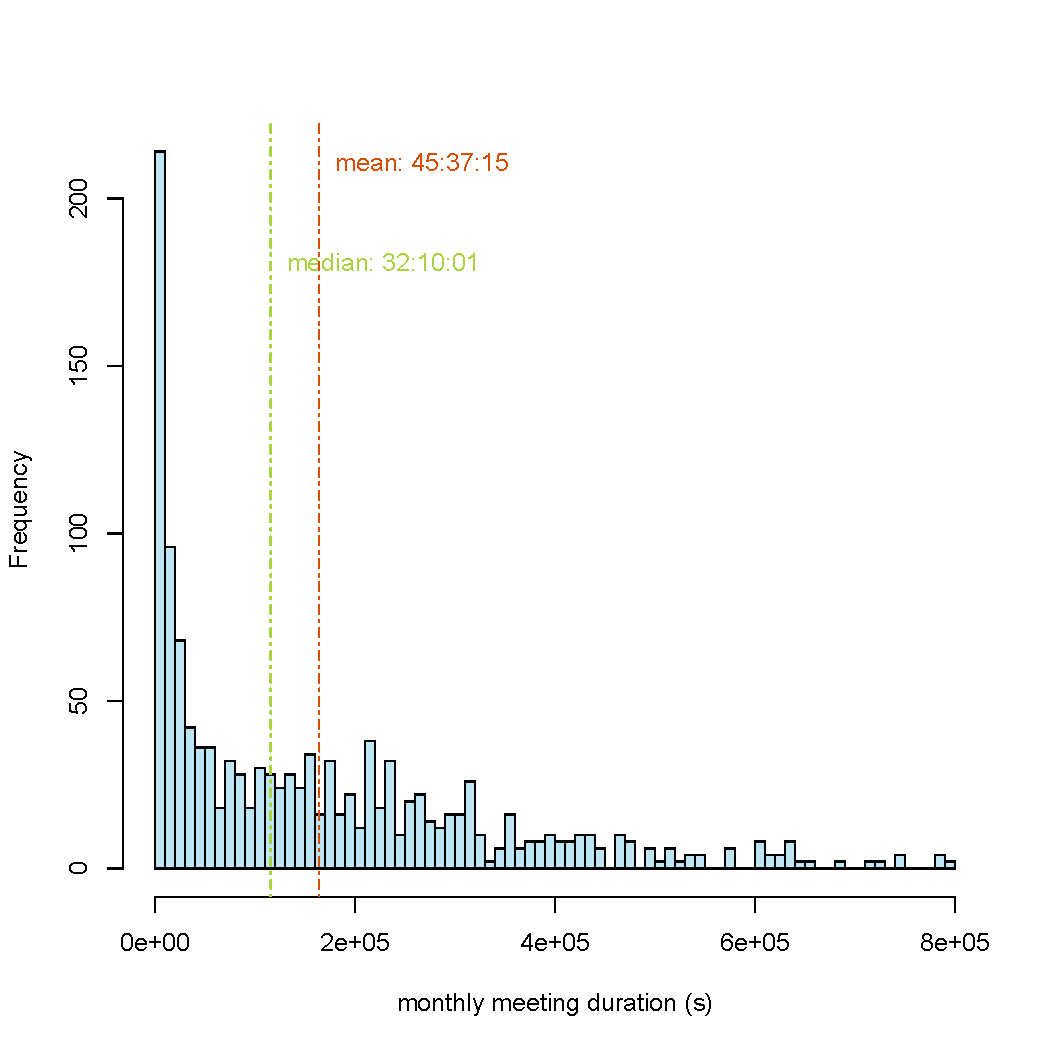
\includegraphics[width=.75\textwidth]{assets/pdf/meeting_frequency_january.pdf}
  \caption[Histogram of monthly meeting duration]{Meeting duration distribution for the network data for January 2009. Additionally, the median and mean values (hh:mm:ss) are indicated.}
  \label{fig:meeting_frequency_januray}
\end{center}
\end{figure}   

\subsection{Visual exploration}
\label{subsec:visual_exploration}

The network visualizations in this section have been created using the \textit{network}\citep{network:08} package, which is part of the \textit{statnet}\citep{statnet:03} library. The layout is determined by the \textit{Fruchterman \& Reingold}\citep{fruchterman:91} algorithm, which is a force directed layouter similar to the one used in the \textit{miceminer} implementation (see section \ref{subsec:graph_explore}).

Other than the visualization in the \textit{miceminer} application, the \textit{network} package allows to visualize all the network components at the same time. Moreover, the package is flexible in terms of the selection of the data to display, or to highlight specific nodes in the visualization.

\subsubsection{General network structure}
\label{subsubsec:vis_general}    

Pictured in figures \ref{fig:graph_january_3h} and  \ref{fig:graph_january_30h} are the networks for January 2009 with the edge filter threshold set to 3 hours and 30 hours, respectively. Although the edges within the components of the network are not visible, the amount of \textit{isolates}, nodes with a degree of zero, is noticeable higher in the network with an edge filter value set to 30 hours. \textit{Isolates} arise from the filter process. Edges with a value lower then the threshold are removed from the network. If all the edges for a certain node are below the threshold, this node becomes an isolate.   

\begin{figure}[htpb]% 
	\centering 
	\subfloat[Network with edge filter set to 3h][Edge filter threshold set to 3 hours.]{
					\label{fig:graph_january_3h} %
					
					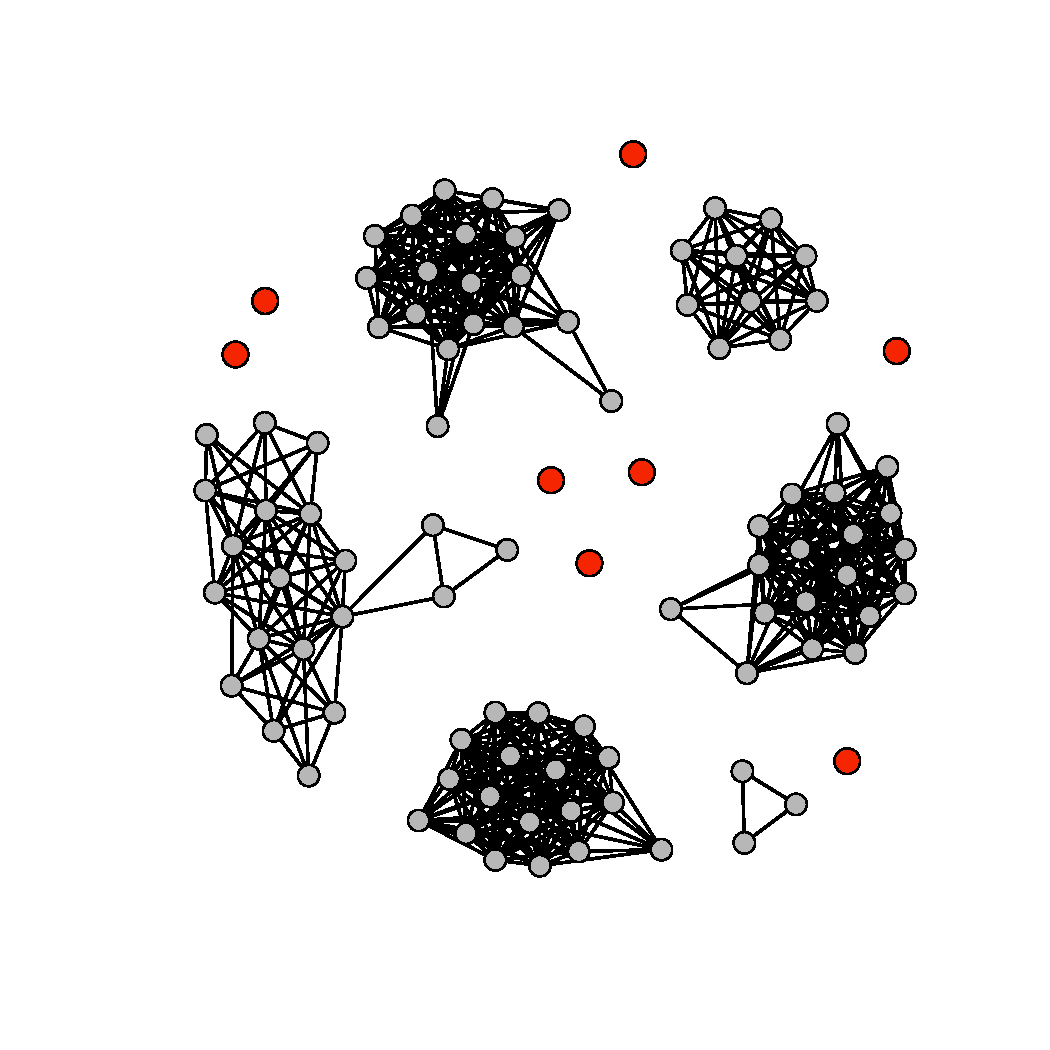
\includegraphics[width=.45\textwidth]{assets/pdf/graph_january_3h.pdf}
				}% 
	\qquad 
	\subfloat[Network with edge filter set to 30h][Edge filter threshold set to 30 hours.]{
					\label{fig:graph_january_30h}%
					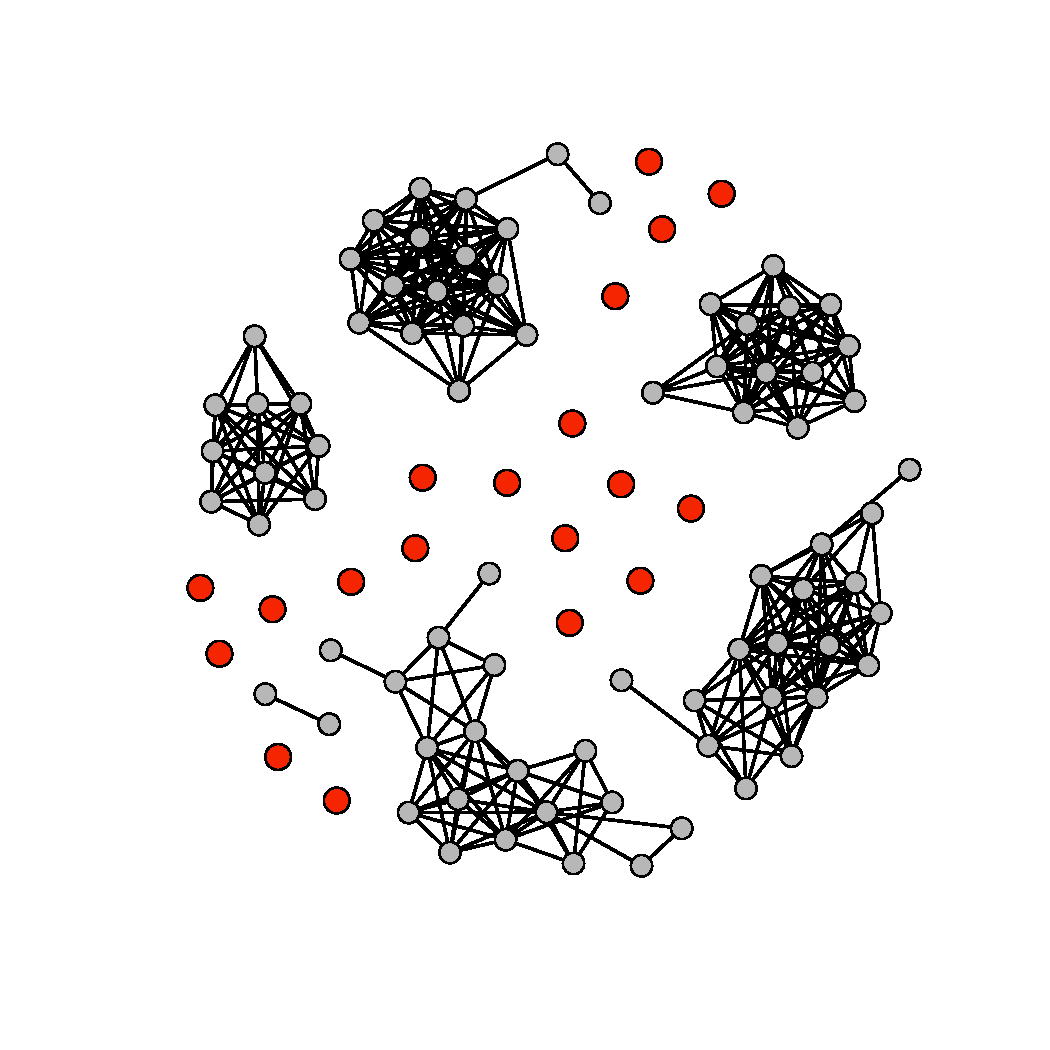
\includegraphics[width=.45\textwidth]{assets/pdf/graph_january_30h.pdf}
				} 
	\caption[Network visualizations with different edge filter values]{A visualization of the network for January 2009 with the edge filter threshold set to 3 hours \subref{fig:graph_january_3h} and 30 hours \subref{fig:graph_january_30h}. Isolates are highlighted red.} 
	 
\end{figure}    

To draw some clearer image of the network and since we are interested in the differences of the inner- and inter-gender networks, the nodes in figures \ref{fig:graph_january_3h_gender} and \ref{fig:graph_january_30h_gender} are colored based on their gender.

\begin{figure}[htpb]% 
	\centering 
	\subfloat[Network with edge filter set to 3h and node coloring based o the gender][Edge filter threshold set to 3 hours.]{
					\label{fig:graph_january_3h_gender} %
					
					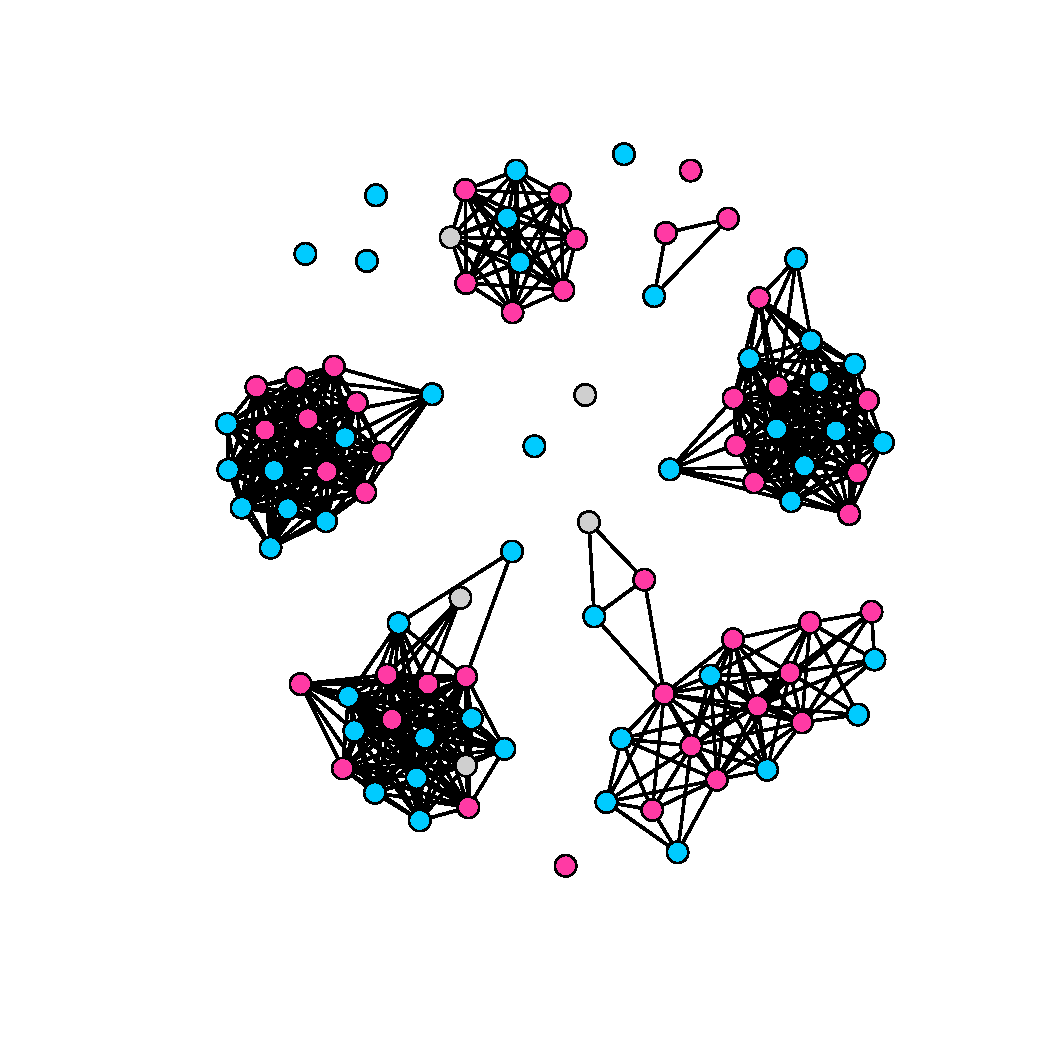
\includegraphics[width=.45\textwidth]{assets/pdf/graph_january_3h_gender.pdf}
				}% 
	\qquad 
	\subfloat[Network with edge filter set to 3h and node coloring based o the gender][Edge filter threshold set to 30 hours.]{
					\label{fig:graph_january_30h_gender}%
					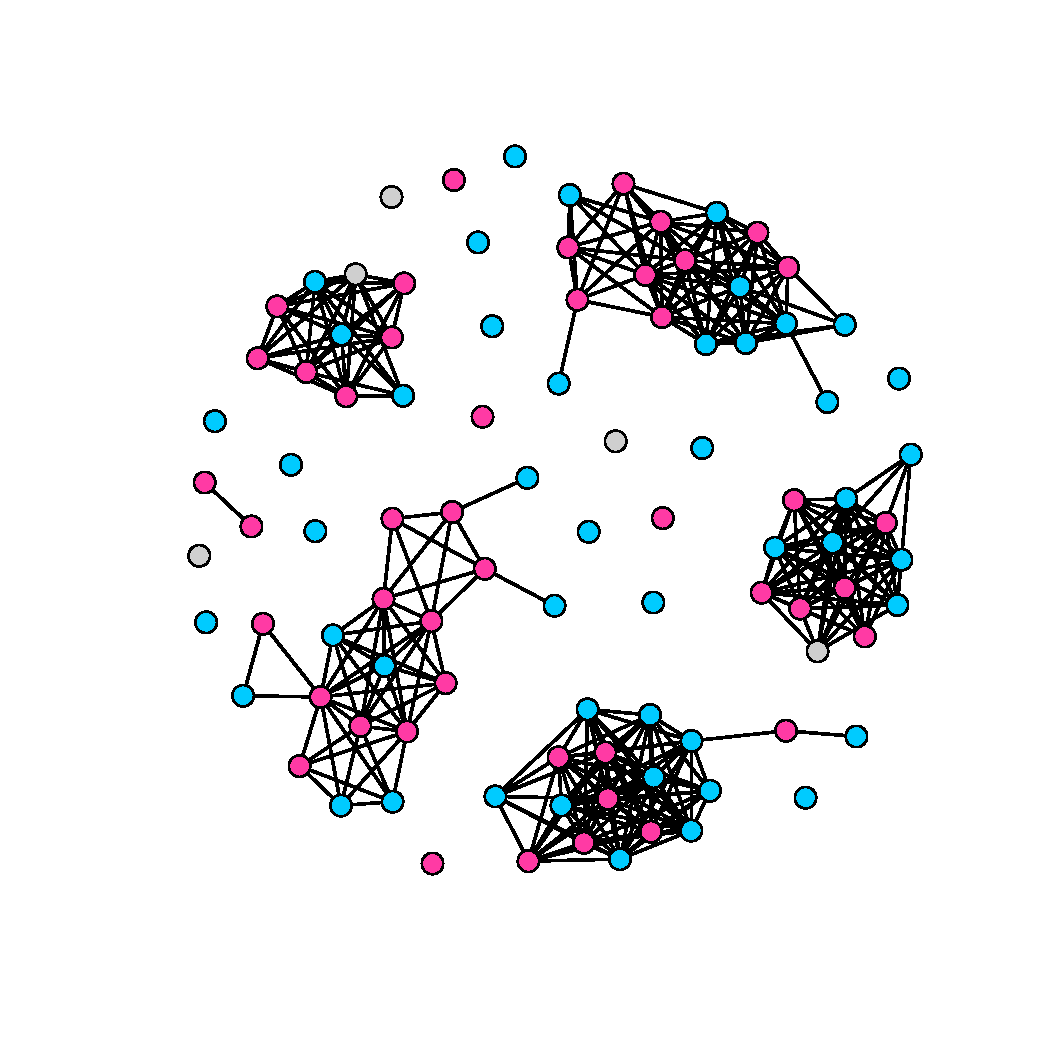
\includegraphics[width=.45\textwidth]{assets/pdf/graph_january_30h_gender.pdf}
				} 
			
	\caption[Network visualizations with different edge filter values]{A visualization of the network for January 2009 with the edge filter threshold set to 3 hours \subref{fig:graph_january_3h} and 30 hours \subref{fig:graph_january_30h}. Additionally, the nodes are colored according to the gender. Female mice are colored pink, males light blue, and mice with an unknown gender grey.} 
	 
\end{figure}

Figure \ref{fig:graph_january_30h_gender} shows, that females tend to be located more in the center of the components, whereas male mice are found in the periphery. Furthermore, the same figure reveals, that the quantity of \textit{isolates} is greater for males than for females. This can be elaborated by visualizing the inner-gender ( see figures \ref{fig:graph_january_30h_ff} and \ref{fig:graph_january_30h_mm} ) and inter-gender (see figure \ref{fig:graph_january_30h_fm}) networks. The visual comparison clearly unveils the higher connectivity within the female mice.

Even in the network with the edge filter set to 30 hours, the entanglement of the edges within the network components do not allow the identification of all individual edges. However, the network filtered with the higher threshold draws a much clearer image of the network structure. For that reason, the following analysis are carried out using the networks with the edge filter set to 30 hours.

\begin{figure}[htpb]% 
	\centering 
	\subfloat[Network of female mice][Network of female mice]{
					\label{fig:graph_january_30h_ff} %
					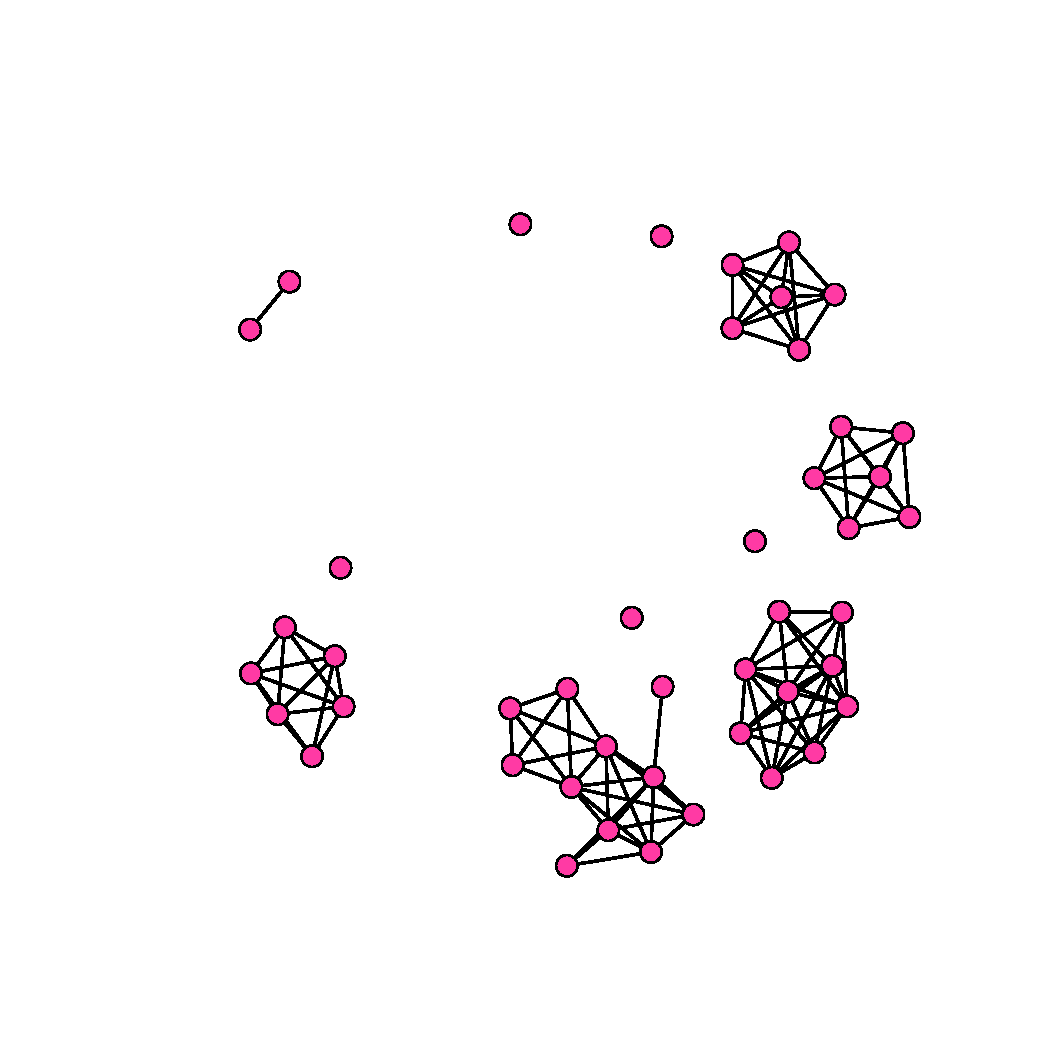
\includegraphics[width=.45\textwidth]{assets/pdf/graph_january_30h_ff.pdf}
				}
	\qquad 
	\subfloat[Network of male mice][Network of male mice]{
					\label{fig:graph_january_30h_mm}%
					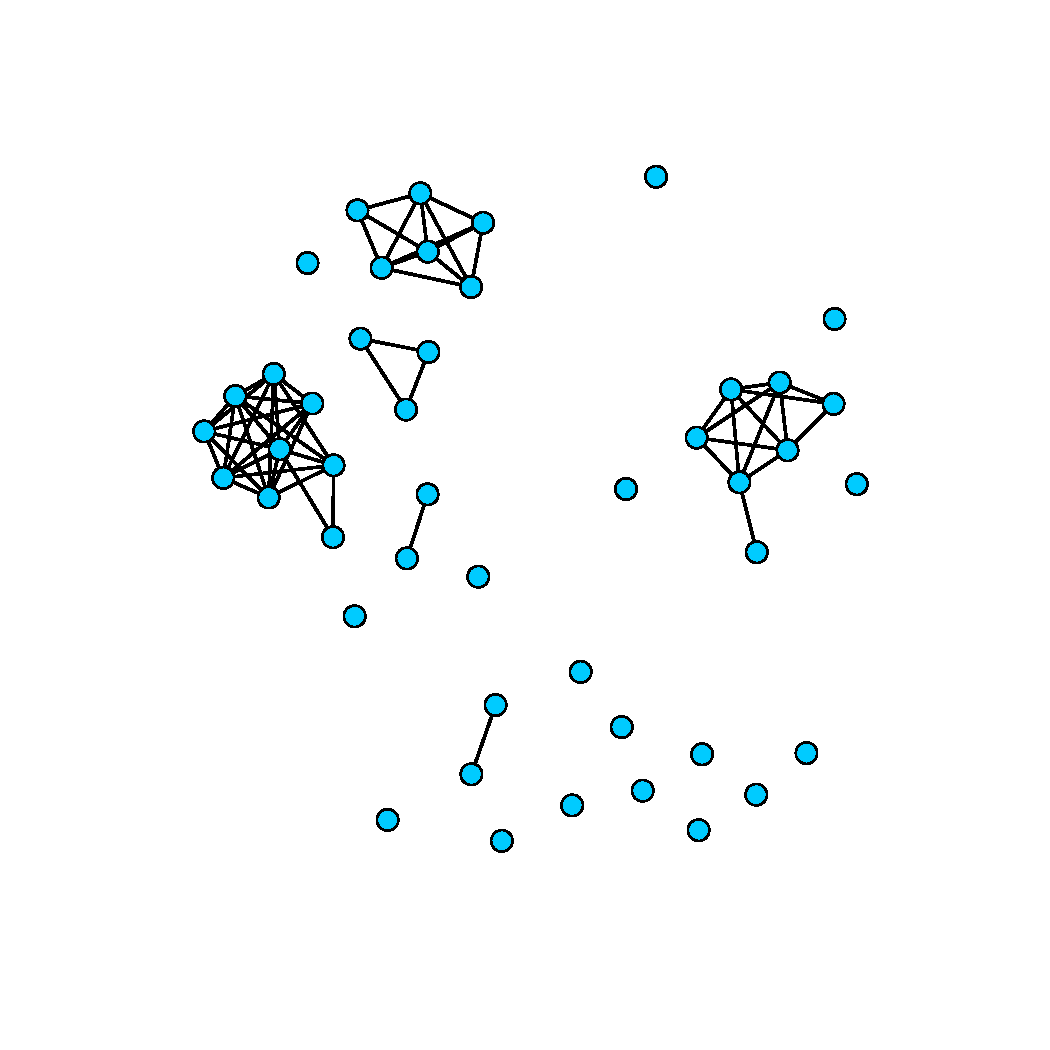
\includegraphics[width=.45\textwidth]{assets/pdf/graph_january_30h_mm.pdf}
				}
	\qquad  
	\subfloat[Inter-gender network][Inter-gender network]{
					\label{fig:graph_january_30h_fm}%
					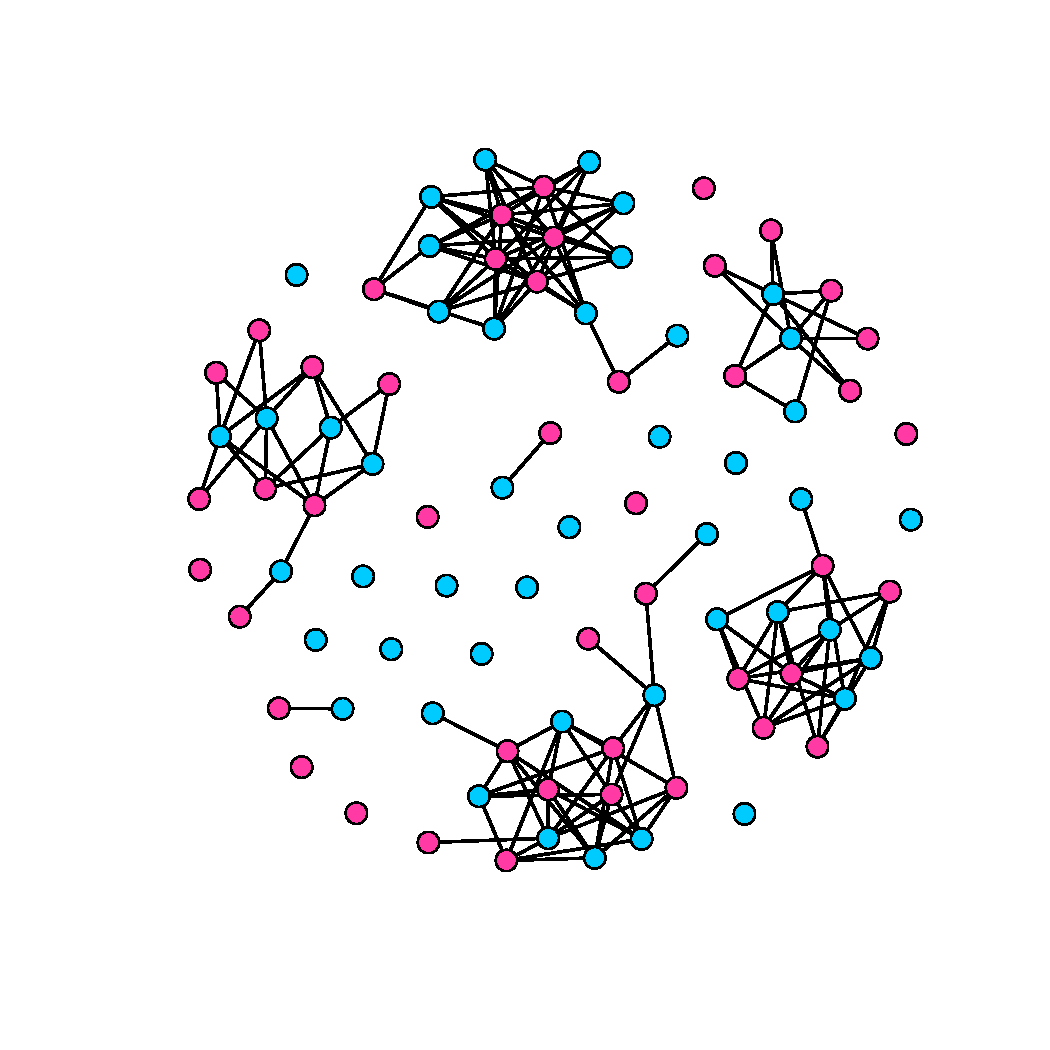
\includegraphics[width=.45\textwidth]{assets/pdf/graph_january_30h_fm.pdf}
				} 
				
	\caption[Network visualizations of the inner- and inter-gender networks]{Visualizations of the inter- and inner-gender networks for January 2009 with the edge filter value set to 30 hours.}
	\label{fig:inner_inter_gender} 
	 
\end{figure}

\subsubsection{Identifying individuals}
\label{subsubsec:vis_individuals}    

After visually examining the general network structure, the visualizations in figure \ref{fig:graph_january_30h_node_based_measures} are adapted to emphasize the role of the individual nodes in the network, based on the node based measures introduced in section \ref{subsec:node_based}. 

\begin{figure}[htpb]% 
	\centering 
				
	\subfloat[Network visualization where the node size is proportional to the average path length of the node][Network visualization where the node size is proportional to the average path length of the node (larger node size means lower value).]{
					\label{fig:graph_january_30h_apl}%
					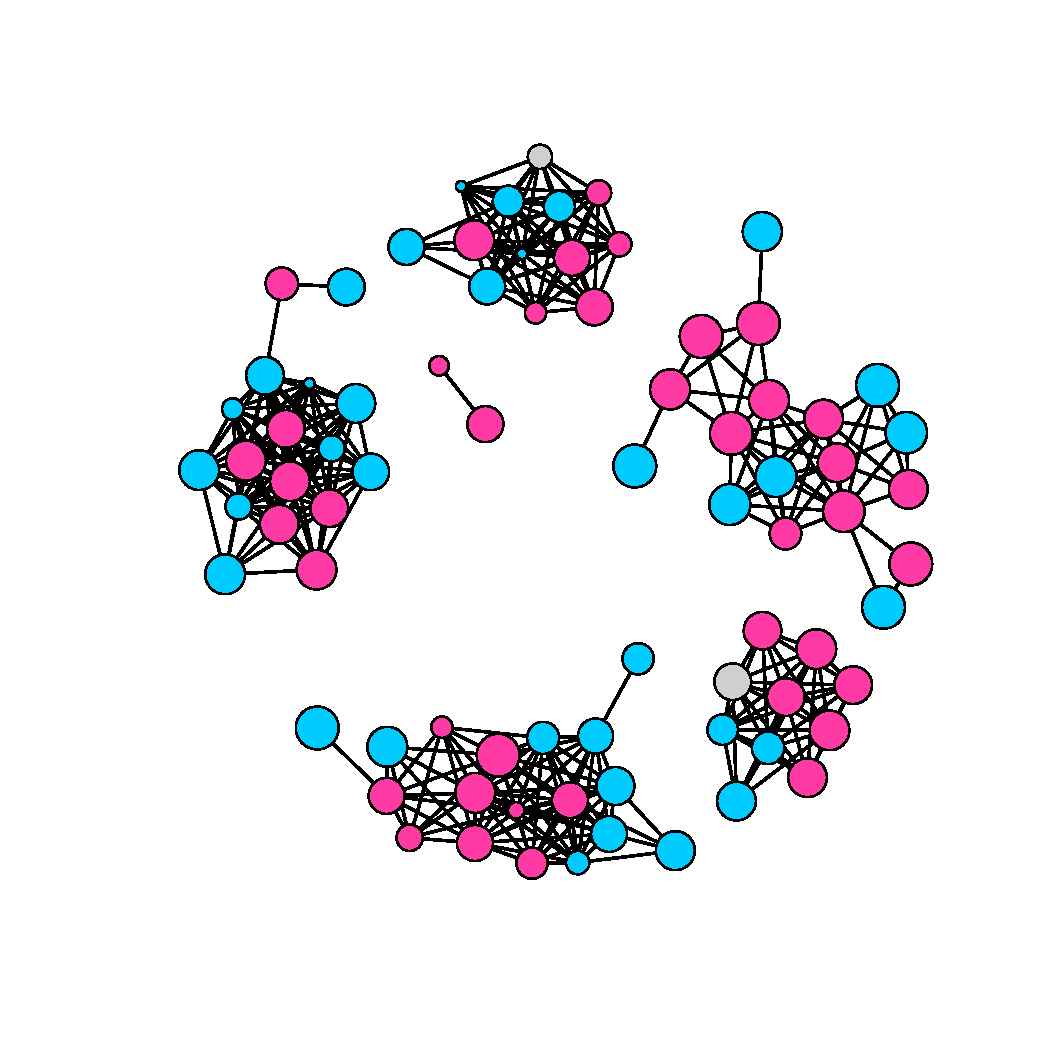
\includegraphics[width=.45\textwidth]{assets/pdf/graph_january_30h_apl.pdf}
				}
	\qquad 
	\subfloat[Network visualization where the node size is proportional to the clustering coefficient of the node][Network visualization where the node size is proportional to the clustering coefficient of the node.]{
					\label{fig:graph_january_30h_cc}%
					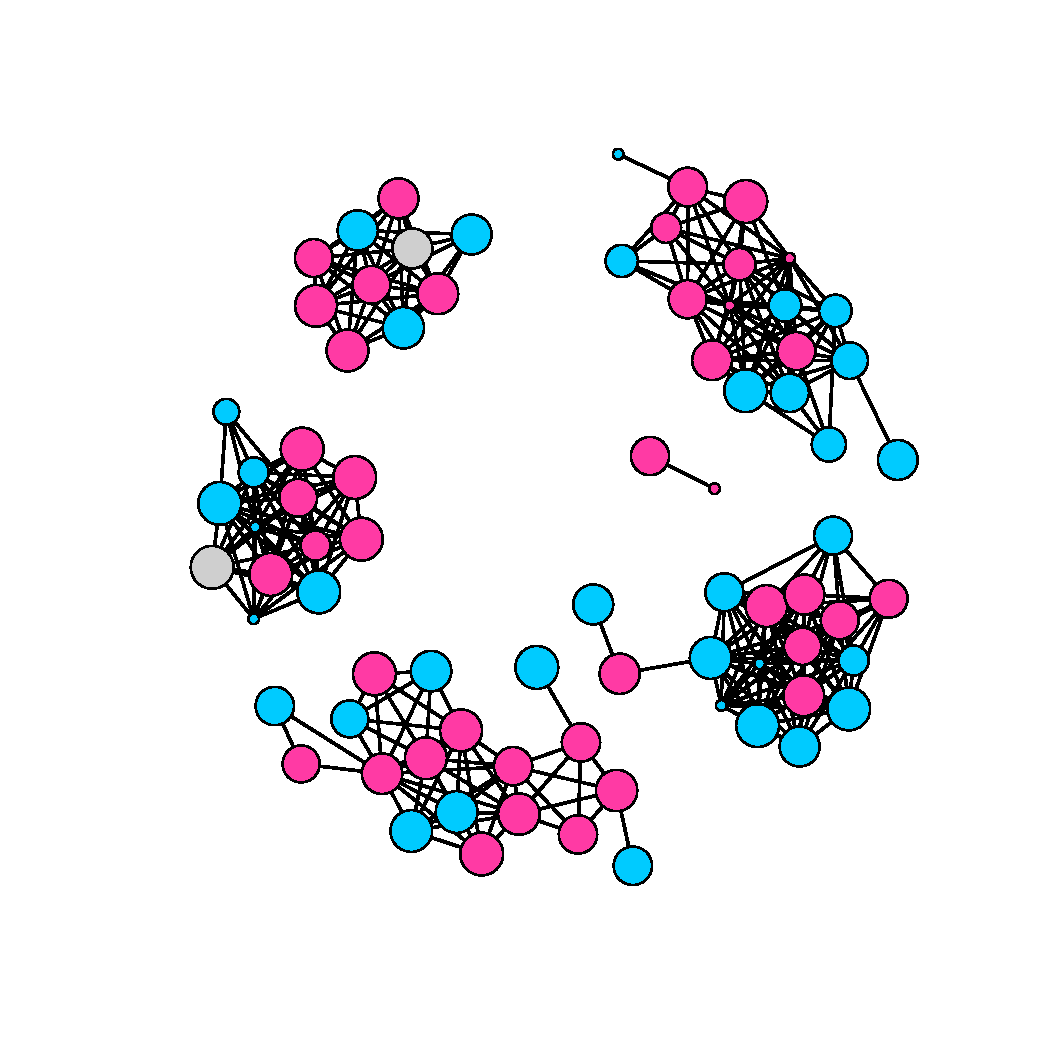
\includegraphics[width=.45\textwidth]{assets/pdf/graph_january_30h_cc.pdf}
				}
	\qquad 			
	\subfloat[Network visualization where the node size is proportional to the degree of the node][Network visualization where the node size is proportional to the degree of the node.]{
					\label{fig:graph_january_30h_degree}
					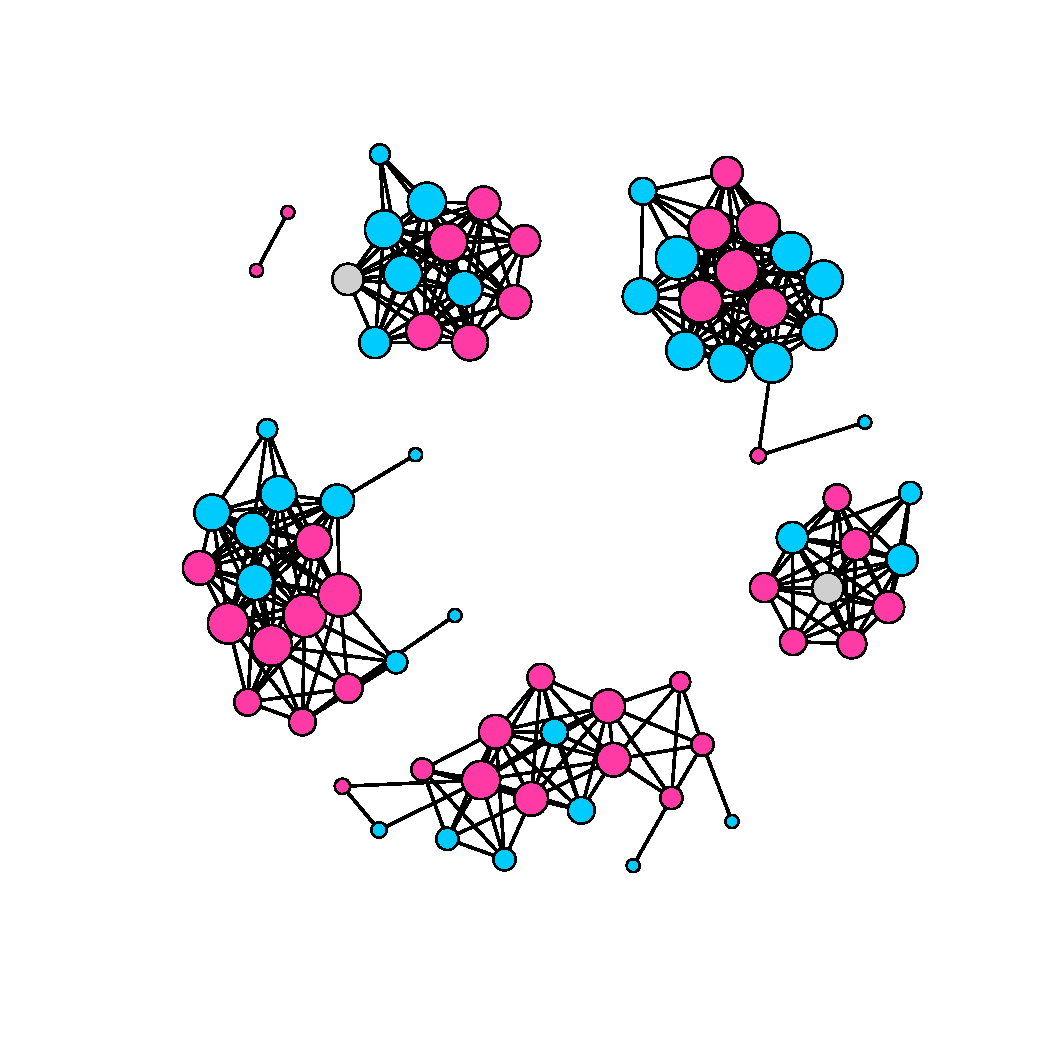
\includegraphics[width=.45\textwidth]{assets/pdf/graph_january_30h_degree.pdf}
				}
	\qquad 
	\subfloat[Network visualization where the node size is proportional to the betweenness of the node][Network visualization where the node size is proportional to the betweenness of the node.]{
					\label{fig:graph_january_30h_betweenness}
					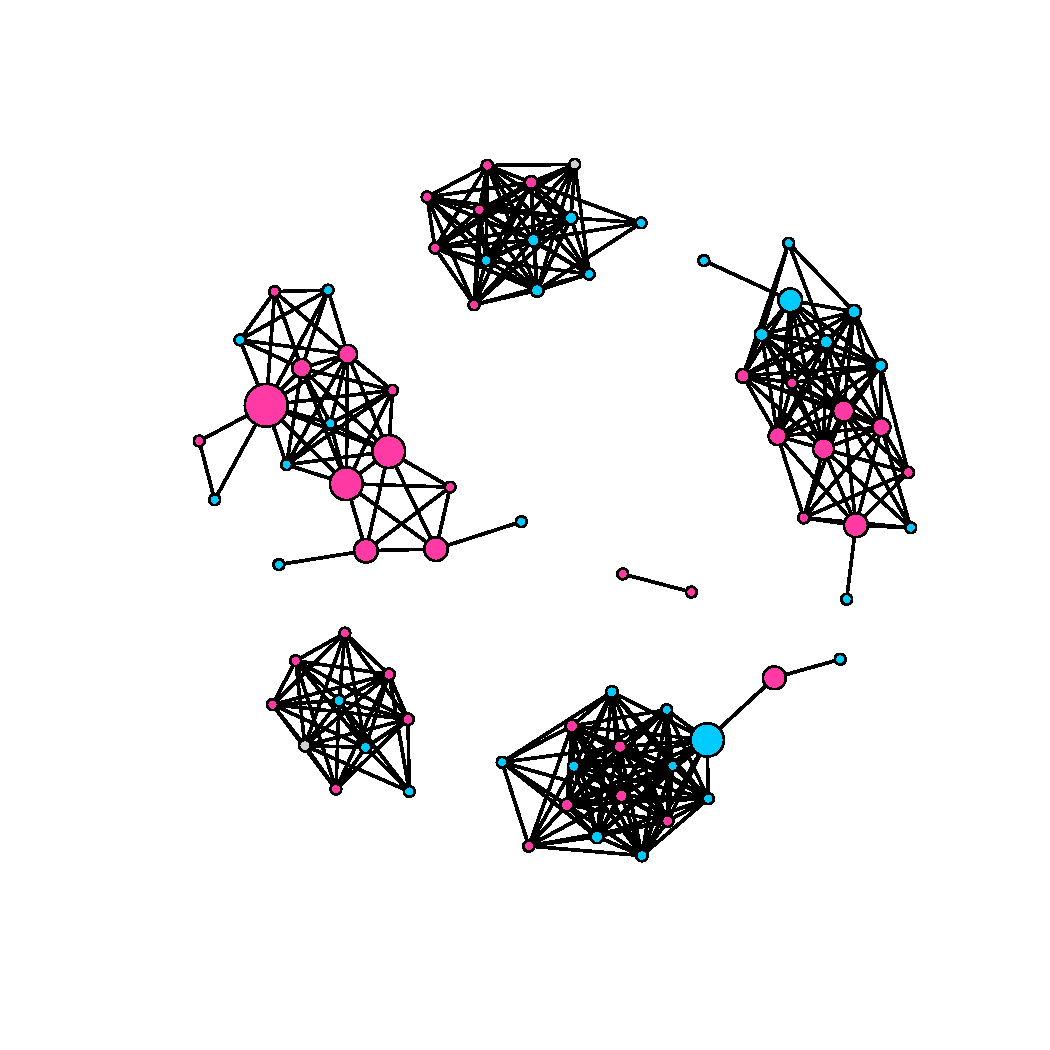
\includegraphics[width=.45\textwidth]{assets/pdf/graph_january_30h_betweenness.pdf}
				} 		 				
		
	\caption[Network visualizations where the node size is proportional to node based measures]{Network visualizations for January 2009, where the node size is proportional to a node based measure.}
	\label{fig:graph_january_30h_node_based_measures} 
	 
\end{figure}

In all but the visualization of the betweenness (figure \ref{fig:graph_january_30h_betweenness}), no nodes stand out. This is coherent to the observation, that the network components are strongly connected. Consequently, the clustering coefficient is generally high, and the average path lengths are low.  

A closer look at figure \ref{fig:graph_january_30h_betweenness}, however, reveals, that most of the nodes with a high betweenness value are \textit{Cut-Points} as well. A \textit{Cut-Point} is a node whose deletion increase the number number of components in the network\citep{pajek:03}. In and of itself, these nodes are very interesting, since they act as a bottleneck when information has to be passed from one sub-network to the other. In this case, however, all the \textit{Cut-Points} connect at most two other nodes to a component (see figure \ref{fig:graph_january_3h_cutpoints}), which reduces their general importance. Hence, we focus on the nodes with a high betweenness value, which are not \textit{Cut-Points} of the kind just explained. The resulting visualization (see figure \ref{fig:graph_january_3h_cutpoints_betweenness}) unveils two female mice with a potentially important position in the network. 

\begin{figure}[htpb]% 
	\centering 
	\subfloat[Network visualization with highlighted \textit{Cut-Points}][Network visualizations for January 2009 with highlighted \textit{Cut-Points}.] {
		\label{fig:graph_january_3h_cutpoints}
  		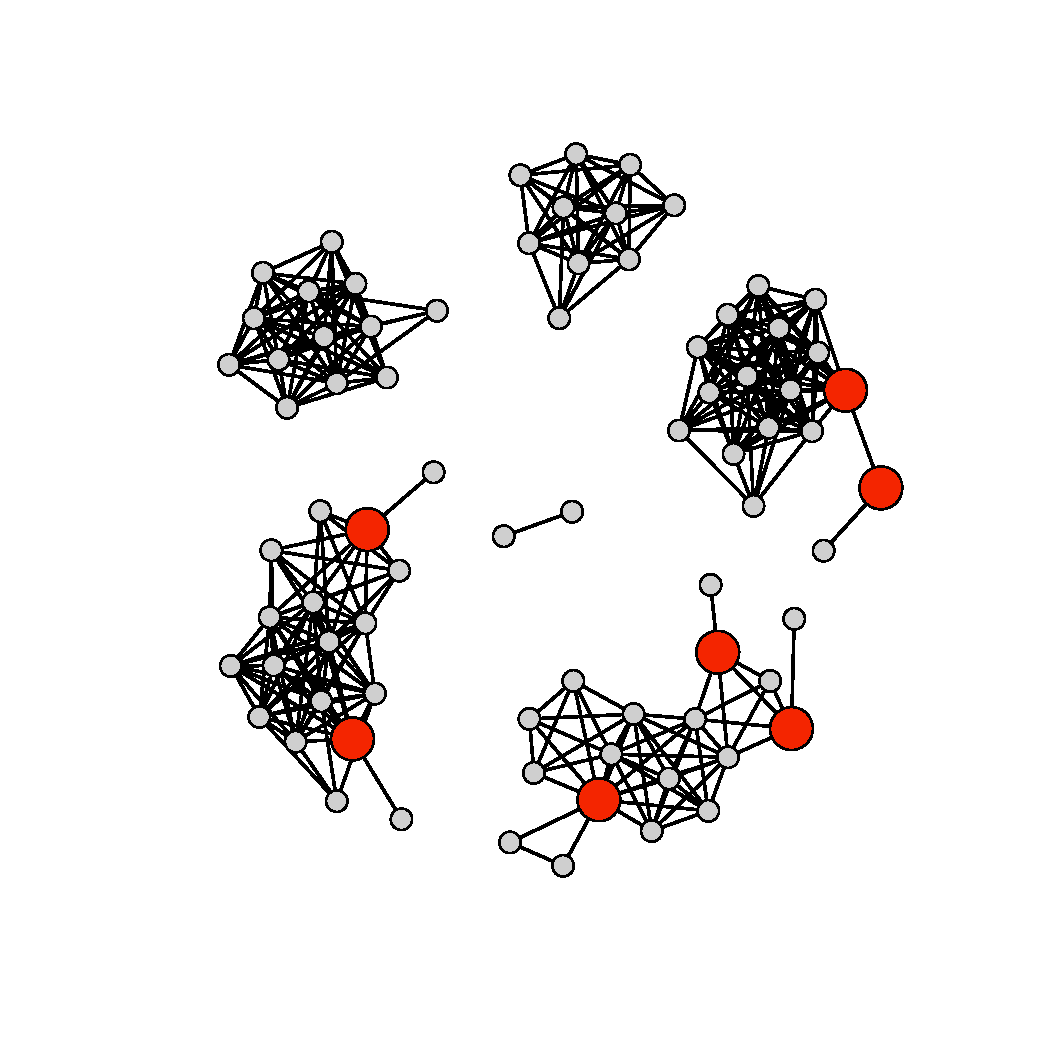
\includegraphics[width=.45\textwidth]{assets/pdf/graph_january_30h_cutpoints.pdf}
	}
	\qquad
	\subfloat[Network visualization with nodes highlighted, that have a high betweenness value and are not \textit{Cut-Points}][The larger nodes have a high betweenness value but are not \textit{Cut-Points}.] {
 		\label{fig:graph_january_3h_cutpoints_betweenness}
 		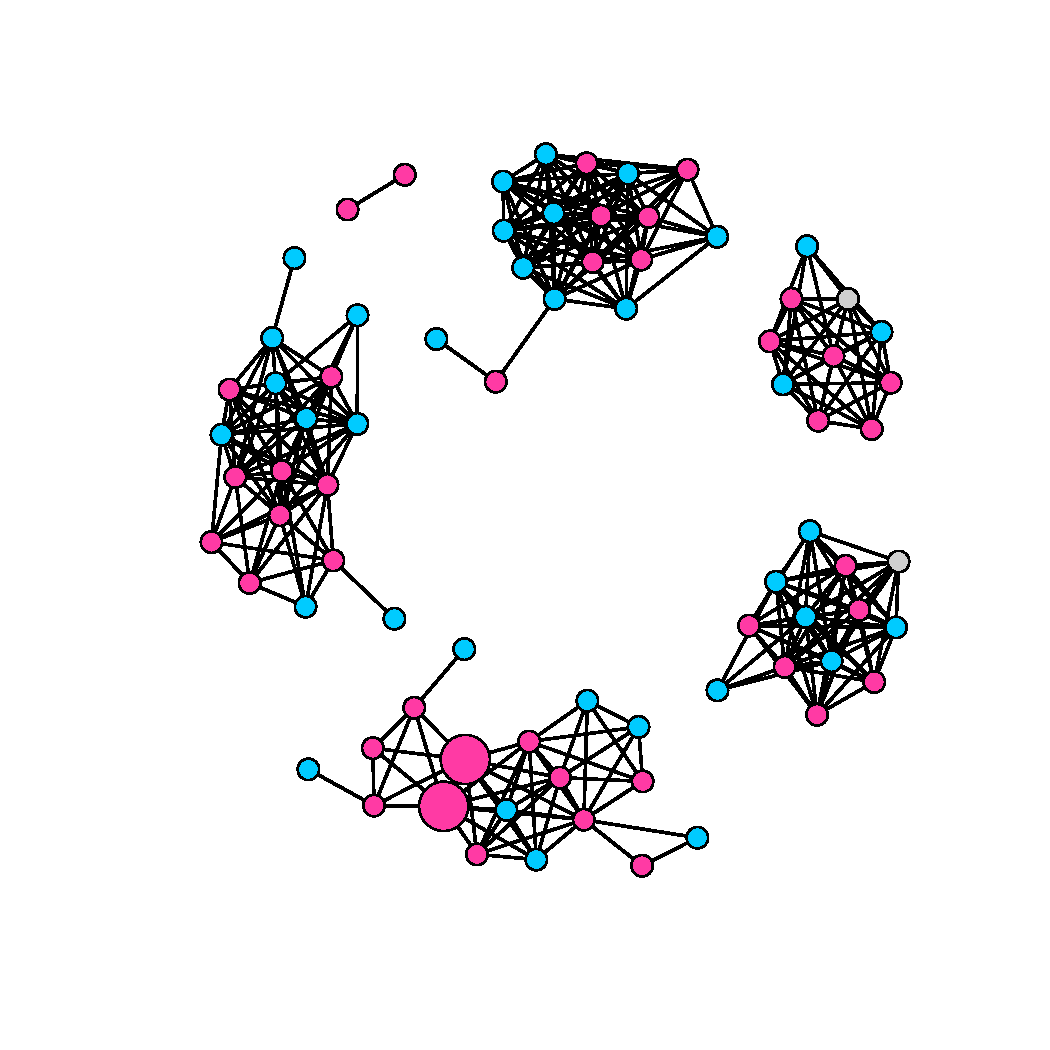
\includegraphics[width=.45\textwidth]{assets/pdf/graph_january_30h_cp_bet.pdf}
  	}
  	
  	\caption[Network visualization of \textit{Cut-Points} and such with a high betweenness value which are not \textit{Cut-Points}]{Identifying \textit{Cut-Points} \subref{fig:graph_january_3h_cutpoints} and such nodes with a high betweenness value which are not \textit{Cut-Points}~\subref{fig:graph_january_3h_cutpoints_betweenness}.}
  	
\end{figure}


\subsection{Quantitative analysis}
\label{subsec:quantitative_analysis}

Aside of quantifying the node based measures, which has already been done for the visualizations, studying the distribution and mixing of these measures allow insights in the mechanisms that led to an observed network structure.  

\subsubsection{General network structure}
\label{subsubsec:general_structure}

A basic question, if we consider the network depicted in figure \ref{fig:graph_january_30h_gender}, is how the separation of the network in several components evolved. To explore this topic, it was determined in which nestboxes the meetings occurred in January 2009. These findings can be mapped to the components found in the network. The results are shown in table \ref{tab:comp_box_meet_dist}.

\begin{table}
\begin{center}
\small
\begin{tabular}{lll}
\hline
\textbf{Component size} &	\textbf{Nestboxes in which the meetings occurred}	&	\textbf{Sum of meeting durations (h:m:s)} \\\hline
18	& 15	& 2006:35:05 \\
 	& 18	& 1800:24:34 \\
	& 13	& 1630:43:24 \\
	& 12	& 1507:04:51 \\
	& 11	& 36:26:24 \\
	& 16	& 00:21:05 \\
	& 17	& 00:16:42 \\
	& 09	& 00:01:31 \\\hline

18	& 27	& 2735:14:47 \\
	& 21	& 950:02:00 \\
	& 29	& 713:50:05 \\
	& 25	& 187:48:39 \\
	& 28	& 141:33:31 \\
	& 22	& 134:26:27 \\
	& 23 	& 12:36:56 \\
	& 24	& 11:02:57 \\\hline

17	& 36	& 5676:16:38 \\
	& 37	& 1716:46:11 \\
	& 35	& 254:34:27 \\
	& 34	& 228:01:20 \\
	& 40	& 179:18:27 \\
	& 38	& 23:19:02 \\
	& 09	& 00:00:12 \\
	& 39	& 00:00:8 \\\hline

13	& 09	& 2339:51:41 \\
	& 08 	& 1984:33:2 \\
	& 10	& 232:50:42 \\
	& 05	& 11:01:31 \\
	& 03 	& 02:05:59 \\
	& 11 	& 00:57:41 \\
	& 06	& 00:12:20 \\
	& 07	& 00:02:50 \\\hline
	
10	& 02	& 2667:49:11 \\
	& 01	& 2075:11:12 \\
	& 04	& 01:26:32 \\
	& 03	& 00:00:32 \\
	& 12	& 00:00:32 \\
	& 09	& 00:00:05 \\\hline

2	& 19	& 52:41:08 \\
	& 20	& 05:08:17 \\
	& 18	& 00:00:30 \\\hline

\end{tabular}
\captionof{table}{Allocation of the nestboxes, in which meetings occurred in January 2009, to the components observed in the network. Additionally the size of the components (number of mice making up the component) and the sum of the meeting durations for the boxes is included (according to the \lstinline|<maxStay>| value explained in section \ref{subsec:miceminer_config}, meetings with a duration of stay longer than 9 hours have been excluded from the sum).}
\label{tab:comp_box_meet_dist}
\end{center}
\end{table} 

Interestingly, if we compare this allocation to the placement of the nestboxes and dividers in the barn (see figure \ref{fig:shedschema} on page \ref{fig:shedschema}), from the six components, five are restricted to one of the four segments (A, B, C, D). Furthermore, the number of boxes where most of the meetings of a component occur (based on the sum of the stay duration), is between 2 and 4. 
 
\subsubsection{Separation of node based measures by gender}
\label{subsubsec:nbm_dist}

Pictured in figure \ref{fig:node_based:measures_dist} are the frequency distributions of the node based measures for female and male mice. An analysis of the segregation of these values by the gender contributes to the understanding of the underlying mechanisms, that form the network.

\begin{figure}[htpb]% 
	\centering 
				
	\subfloat[Average path length]{
					\label{fig:graph_january_30h_apl_dist}%
					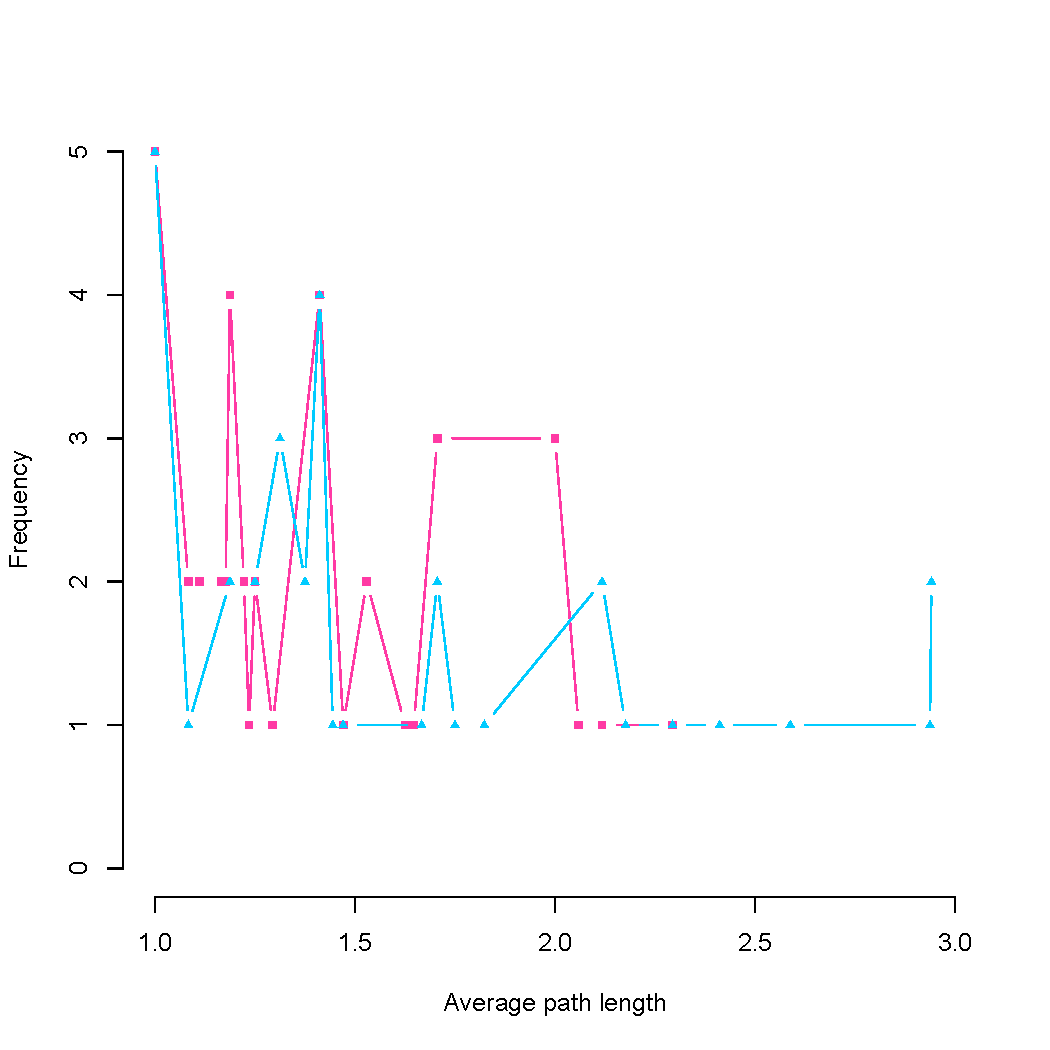
\includegraphics[width=.45\textwidth]{assets/pdf/graph_january_30h_apl_dist.pdf}
				}
	\qquad 
	\subfloat[Clustering coefficient]{
					\label{fig:graph_january_30h_cc_dist}%
					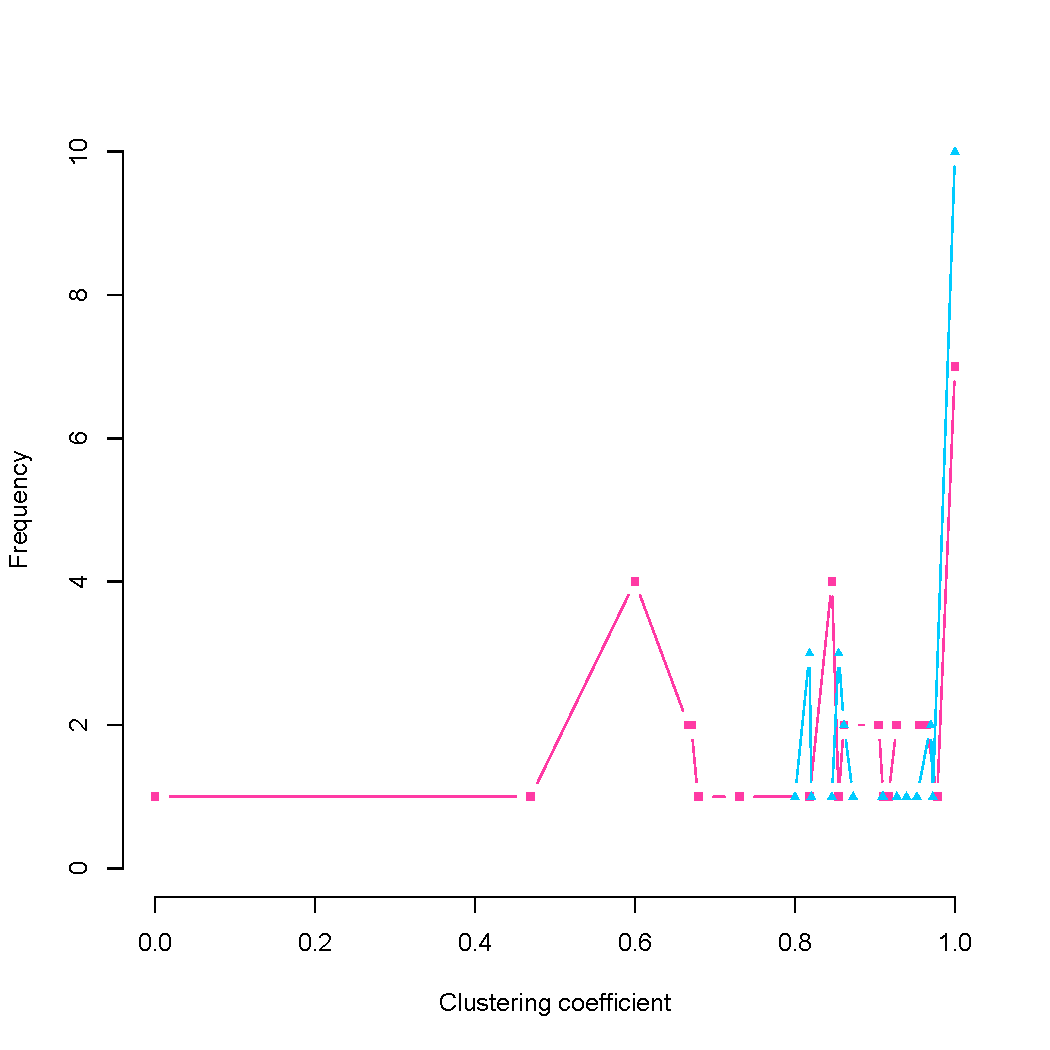
\includegraphics[width=.45\textwidth]{assets/pdf/graph_january_30h_cc_dist.pdf}
				}
	\qquad 			
	\subfloat[Degree]{
					\label{fig:graph_january_30h_degree_dist}
					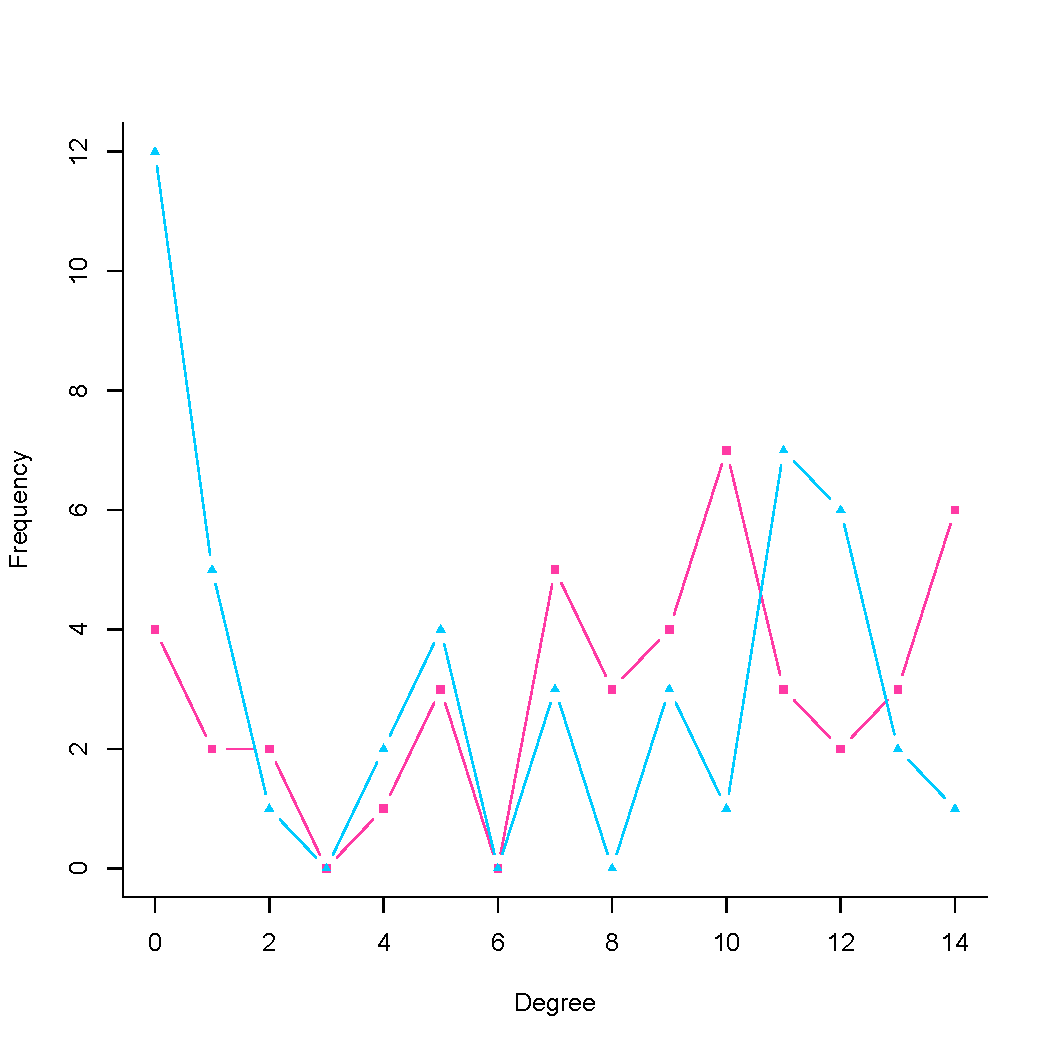
\includegraphics[width=.45\textwidth]{assets/pdf/graph_january_30h_degree_dist.pdf}
				}
	\qquad 
	\subfloat[Betweenness]{
					\label{fig:graph_january_30h_betweenness_dist}
					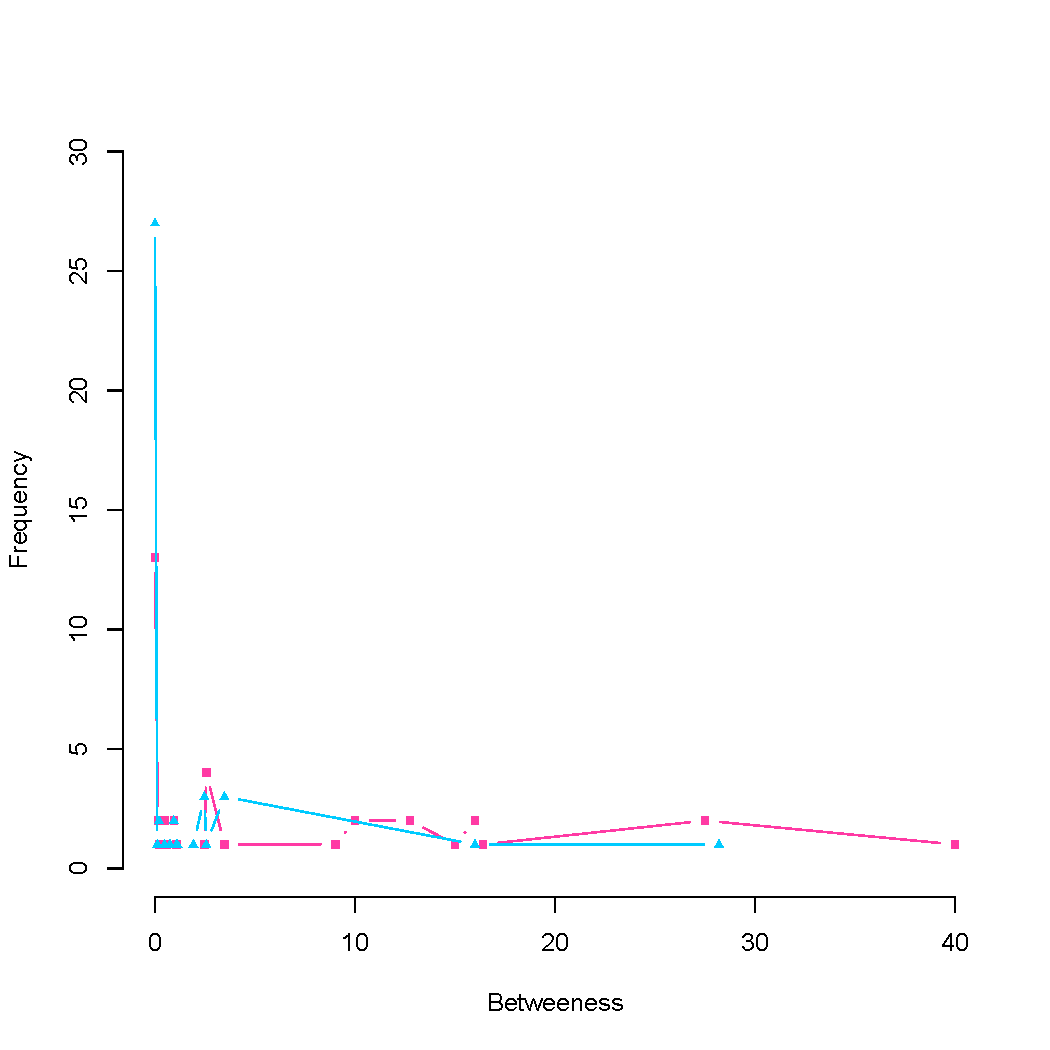
\includegraphics[width=.45\textwidth]{assets/pdf/graph_january_30h_bet_dist.pdf}
				} 		 				
				
	\caption[Distribution of the node based measures split up by the gender.]{Distribution of the node based measures, for the network data of January 2009 with an edge filter value of 30 hours. Values for female mice are colored pink and light blue for males.}
	 \label{fig:node_based:measures_dist}
\end{figure}

Although the charts do not show a clear separation, the observations made in the network visualizations (figures \ref{fig:inner_inter_gender} and \ref{fig:graph_january_30h_node_based_measures}), that females are better connected, is supported. Figure \ref{fig:graph_january_30h_degree_dist}, for instance, shows, that there are more male \textit{isolates} than female. Furthermore, the female mice with a high betweenness value are easy seen in figure \ref{fig:graph_january_30h_betweenness_dist}. 

The simplest way to quantify the segmentation, is to calculate the means by gender (see table \ref{tab:means_nbm}). There seems to be an explicit difference in the betweenness and the degree values. 
\begin{table}
\begin{center}
\begin{tabular}{l+lll}
\toprule
\textbf{Node based measure} &	\textbf{Mean females}	&	\textbf{Mean males}	& \textbf{range of values (min /max) } \\\midrule
Average path length	& 1.27	& 1.22	&  1 / 2.94 \\
Clustering coefficient	& 0.70	& 0.59	& 0 / 1 \\
Degree	& 8.2	& 6	& 1 / 14 \\
Betweenness	& 5.43	& 1.54	& 0 / 40 \\\bottomrule
\end{tabular}
\captionof{table}{Mean values of the node based measures separated by gender. Additionally the range of the values is indicated.}
\label{tab:means_nbm}
\end{center}
\end{table}

However, a better method to determine the separation of these values by gender, is to use a \textit{Mann-Whitney} test\citep{siegel:88}. For this test, all values for a node based measure, are arranged into a single ranked series. 

Let $R_f$ denote the ranks of females in this series, and $n_f$ , $n_m$ be the numbers of female and male nodes. The equation to get the coefficient $U_f$ looks like

\begin{equation}
U_f = n_fn_m\frac{n_f(n_f + 1)}{2} - R_f
\label{eq:mann_w}
\end{equation}  

$U_f$ is then scaled by $n_fn_m$

\begin{equation}
u_f = \frac{U_f}{n_fn_m}
\label{eq:mann_w_norm}
\end{equation}
 
The value for $u_f$ is always between 0 and 1. If females occupy the lowest $n_f$ ranks,  $u_f = 0$, and if males occupy the lowest $n_f$ ranks, $u_f=1$. For a perfect mixing of ranks, $u=0.5$.

The results are listed in table \ref{tab:u_test}. For the calculation of the average path length and the clustering coefficient values, the \textit{isolates} were not included, since they would bias the result.

\begin{table}
\begin{center} 
\renewcommand\arraystretch{1.2}
\begin{tabular}{lllll}
\toprule
\textbf{Measure} &	\textbf{Females}	& \textbf{Males}	& \textbf{$u$} \\\midrule
Average path length	&	41	&	35	& $0.38$\\
Clustering coefficient	&	41	&	35	&  $0.65$ \\
Degree	&	45 	& 	47 	& $0.62$	\\
Betweenness	&	45	&	47	&	$0.67$ \\\bottomrule

\end{tabular}
\captionof{table}{$u$ values for node based measures calculated using a \textit{Mann-Whitney} test.}
\label{tab:u_test}
\end{center}
\end{table}

As well in this values, a tendency for a better connectedness of the female mice is visible. Please note, that lower values for the average path length, means a better rank.

To test whether the calculated values of $u$ are statistical significant, the values would be compared to the ones calculated for a set of random graphs with a fixed degree distribution\citep{croft:07}\citep{newman:02a}. However, no implementation could be found to generate such random networks for unconnected graphs (network which consists of several components).

\subsubsection{Assortativity coefficient}
\label{subsubsec:assortivity}     

The assortativity coefficient\citep{newman:03} is used to measure association patterns in social networks. If $e_{ij}$ is the fraction of edges in the network that connect nodes of type $i$ to nodes of type $j$, the assortativity coefficient is defined as

\begin{equation}
r = \frac{ \sum_i e_{ii} - \sum_{ijk} e_{ik} e_{jk} }{ 1 - \sum_{ijk} e_{ik} e_{jk}}
\label{eq:ass_coeff}
\end{equation} 

where $k$ is a dummy variable used to iterate the sum\citep{lusseau:04}. This quantity equals $1$ when we have perfect assortative mixing, meaning that all nodes of a category are connected to nodes of the same category. For a disassortative mixing, when every node of a type is connected to a node of another category, the value of $r$ lies between $-1 \leq r \leq 0$. 

\paragraph{Gender correlation}
\label{para:gender_corr}

In our data, one category we can test for is the gender. Table \ref{tab:mm} shows the \textit{mixing matrix}, which discloses the quantities of the inner- and inter-gender connections in the network of January 2009 (e.g. there are 154 edges between males and females).

\begin{table}
\begin{center}
\newcolumntype{H}{>{\centering\bf}p{0.3cm}}
\begin{tabular}{+H|^c^c^c}
\rowstyle{\bfseries}
	&	f	&	m	&	u \\\hline
f	&	103	&	154	&	10 \\
m	&	154	&	60	&	8 \\
u	&	10	&	8	&	0 \\	
\end{tabular}
\captionof{table}{The \textit{mixing matrix} of the gender category for the network data of January 2009.}
\label{tab:mm}
\end{center}
\end{table}

This distribution yields to an $r$ value of $0.010$ which implies a disassortative mixing. Edges which contain nodes from which the gender is not known were not included in the calculation.

For a mixing matrix with several categories this value would be tested for statistical significance, for example using the \textit{jackknife}\citep{newman:03} method,  

\begin{equation}
\sigma_r^2 = \sum_{i=1}^M(r_i -r)^2
\label{eq:ass_coeff_gender}
\end{equation}  

where $r_i$ is the $r$ value of the network in which the $i$-th edge is removed, to determine the standard deviation, followed by a simple $t$-test\citep{snijders:99}.

However, this is not applicable for the present data, since the $r$ values calculated according to the \textit{jackknife} method are not subject to Gaussian distribution. Each iteration in the \textit{jackknife} method either removes an inner- or inter-gender edge. Therefore, only three different $r$ values occur.

\paragraph{Degree correlation}
\label{para:degree_corr}
 
Another form of assortative mixing is the degree correlation, which is used to measure the assortative mixing by the node degree. The question behind this value is whether individuals with high degrees tend to be connected to others with a high degree\citep{croft:07}. Calculation of the value for the network of January 2009 using the Pearson correlation, as suggested by \textit{Newman}\citep{newman:02}, results in $r_p = 0.373$. \citep{newman:03a}. 

There is no general interpretation of the value. However, we can compare it with the values calculated for other networks. Interesingly, many social networks exhibit a positive degree correlation, whereas metabolic networks, food webs and neural networks usually have a negativ degree correlation\citep{newman:03a}. \textit{Lusseau et al.}\citep{lusseau:06} for example, reported a value of $r_p = 0.170$ for a social network of bottelnose dolphins, and \textit{Croft et al.}\citep{croft:05} found degree correlation values between $0.28$ and $0.7$ for 5 populations of small freshwater fish.   
 
\subsection{Longitudinal exploration of the network data}
\label{subsec:longitudinal}

After the visual exploration, and the examination of some quantitative network measures on the basis of a single network, we expand this methods to a series of networks. The series includes the data from June 2008 to June 2009. Although this 13 networks do not reveal eventual annual periodicities, as such a study would need to be carried out with network data for several year, tendencies can still be spotted.
 
To identify this tendencies, rather than analysing the data based on known methods to study the longitudinal dynamics in networks\citep{snijders:05}, most of the already introduced quantitive measures have been calculated for the whole set. A possible trend in the dynamics, or another exceptional finding, of a measure is described on spot.

\subsubsection{Nodes}

Pictured in figure \ref{fig:long_node}, is the quantity of mice for each of the thirteen months. These numbers do only include mice for which meetings have been recorded. The blue values indicate the whole amount of mice per month. The values in pink, light blue and grey, represent the quantity of female, male and mice with an unknown gender, respectively. Unless otherwise stipulated, the color code is the same for all of the figures in this section.

Notable is the convergence of the quantities for the female and male mice from September 2008 to April 2009. This allows for a more significant comparison of these networks, since a lot of the methods and measures are in some way dependent on the number of nodes.  

\begin{figure}[htpb]
\begin{center}
  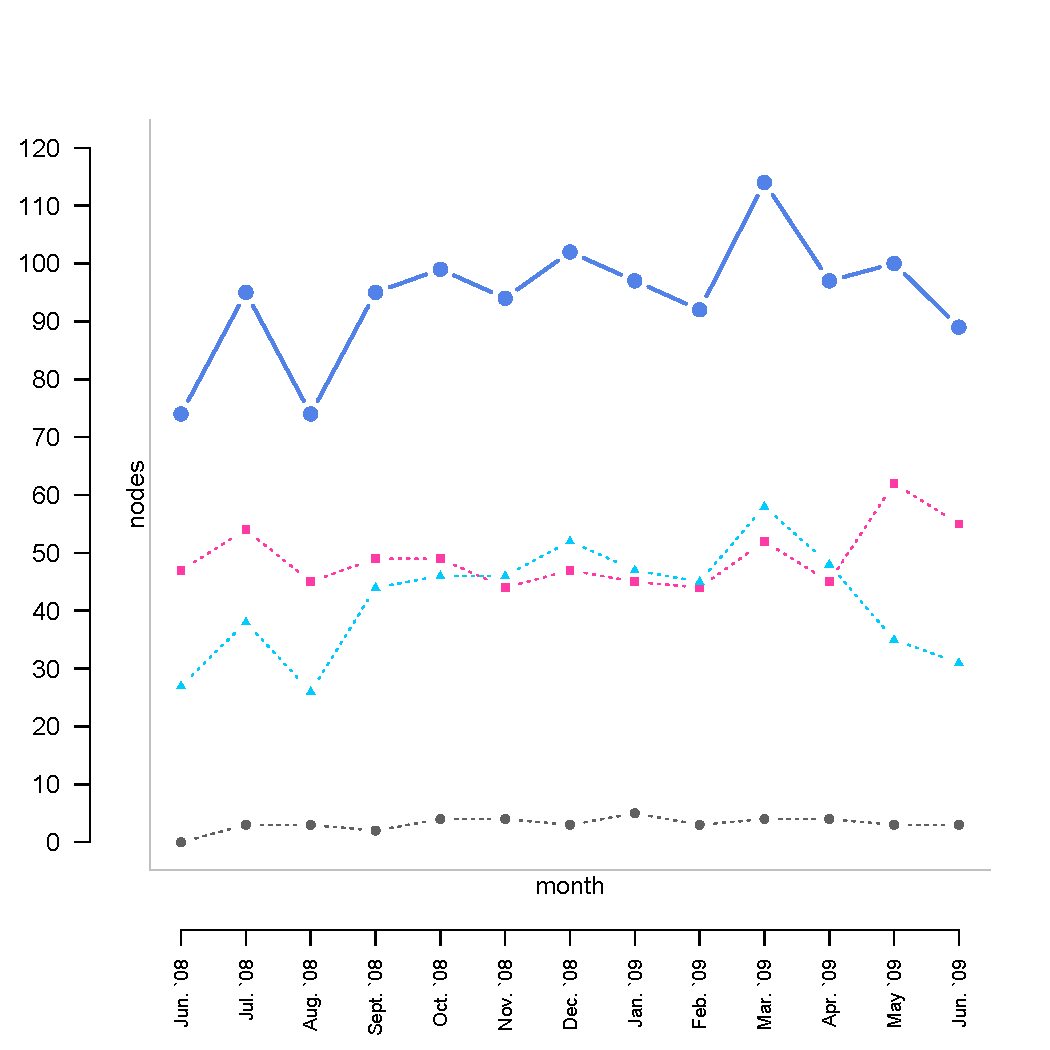
\includegraphics[width=.6\textwidth]{assets/pdf/long_nodes.pdf}
  \caption[Number of mice over the months]{Quantity of mice for each month. The solid blue line indicates the sum of the female (pink), the male (light blue) and the mice with an unknown gender (grey).}
  \label{fig:long_node}
\end{center}
\end{figure}

\subsubsection{Edges}

Figure \ref{fig:long_edges} shows the number of edges for the networks. Furthermore, the number of edges between females (pink), males (light blue), between males and females (grey) are indicated. The sum of the edges (colored blue) does comprehend the edges that includes mice of which the gender is unknown. However, this fraction is not indicated in the figure.

\begin{figure}[htpb]
\begin{center}
  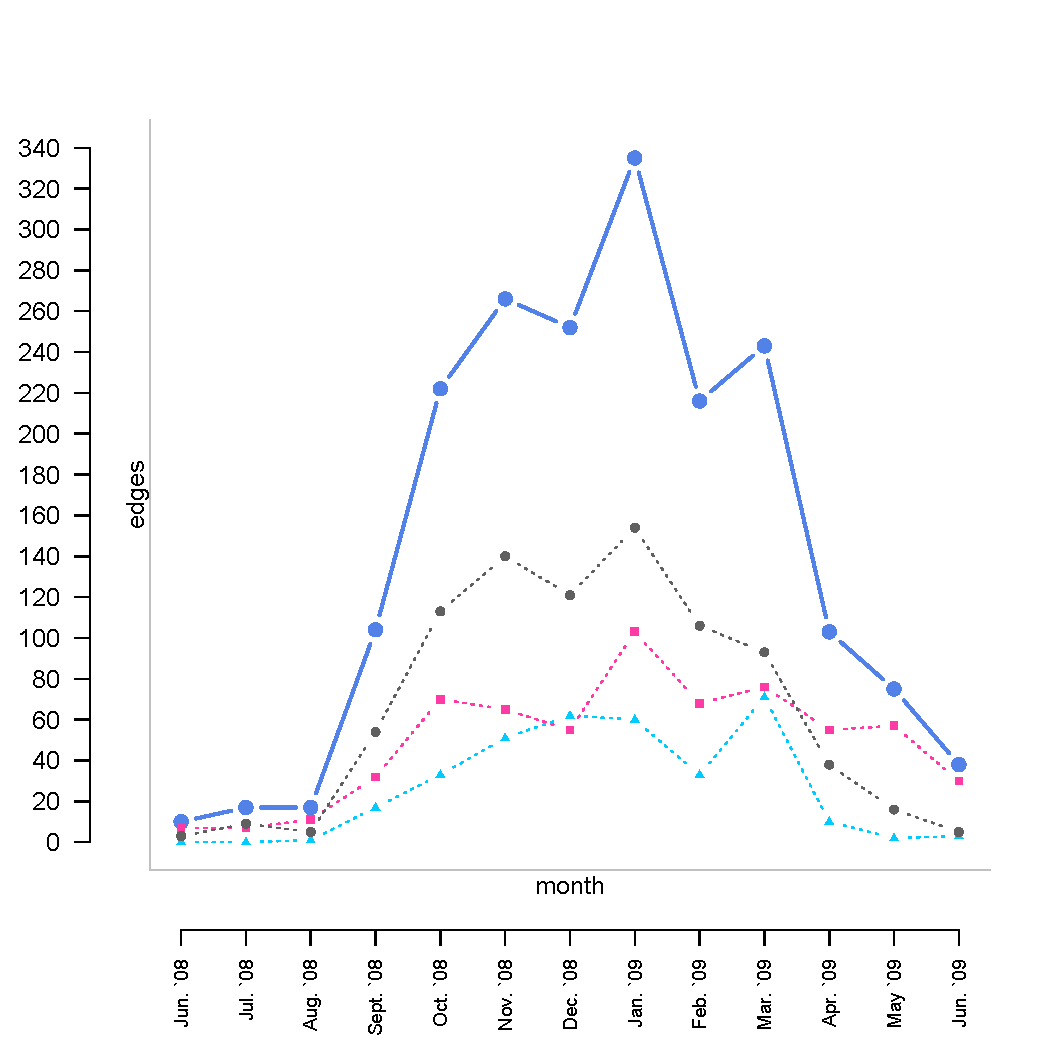
\includegraphics[width=.6\textwidth]{assets/pdf/long_edges.pdf}
  \caption[Number of edges over the months]{Number of edges over the months.}
  \label{fig:long_edges}
\end{center}
\end{figure}

The chart suggests a seasonal trend for the connectedness of the mice during summer and winter. Even though the number of mice is lower in summer than in winter (see figure \ref{fig:long_node}), the differences in the connectedness of the mice is clearly visible when the networks are compared visually. Figure \ref{fig:june_jan_side} shows the networks for June 2008 and January 2009 side by side. Quite clearly, the density of edges in the network for January is much higher than for June. The density of a network can be quantified by calculating the fraction of possible edges in the network, which is given by 

\begin{equation}
\rho = \frac{E}{E_max} = \frac{2E}{n(n-1)}
\label{eq:density}
\end{equation}      

where $E$ denotes the existing edges, and $n$ is the number of nodes in the network. The densities for June 2008 and January 2009 are $\rho_{jun.} = 0.01$ and $\rho_{jan} = 0.14$. The factor of 14 between this two values is even underestimated, since the number of possible edges for June is $2701$\footnote{$E_{max} = (\frac{1}{2})n(n-1) = (\frac{1}{2}) 74(74 -1) = 2701$} whereas for January 2009 it is 4656\footnote{$E_{max} = (\frac{1}{2}) 97(97-1)  = 4656$}. Hence, the mice are much better connected in winter than in summer.  

\begin{figure}[htpb]% 
	\centering 
	
	\subfloat[June 2008]{
					\label{fig:graph_jun_30h}%
					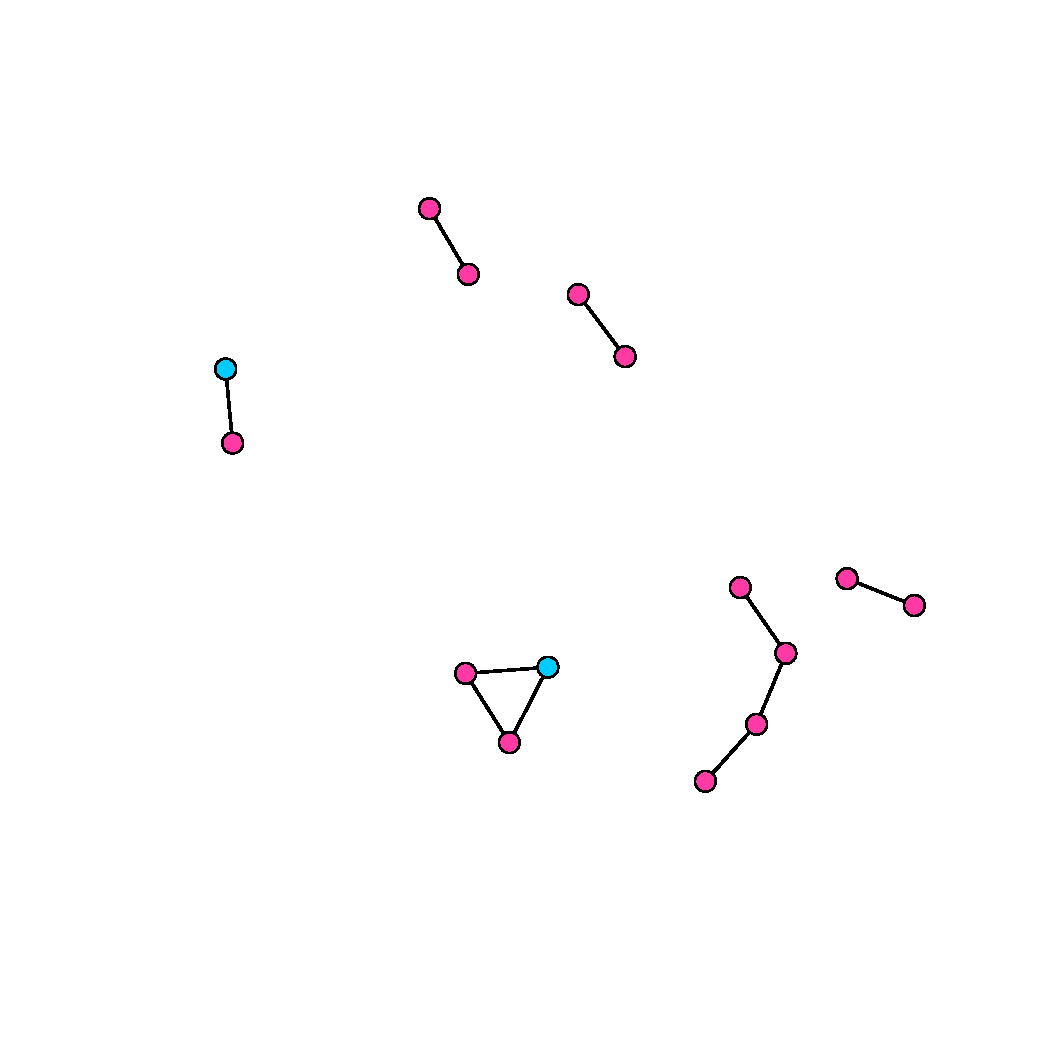
\includegraphics[width=.45\textwidth]{assets/pdf/graph_june_08_30h.pdf}
				}	
	\qquad 			
	\subfloat[January 2009]{
					\label{fig:graph_jan_30h}%
					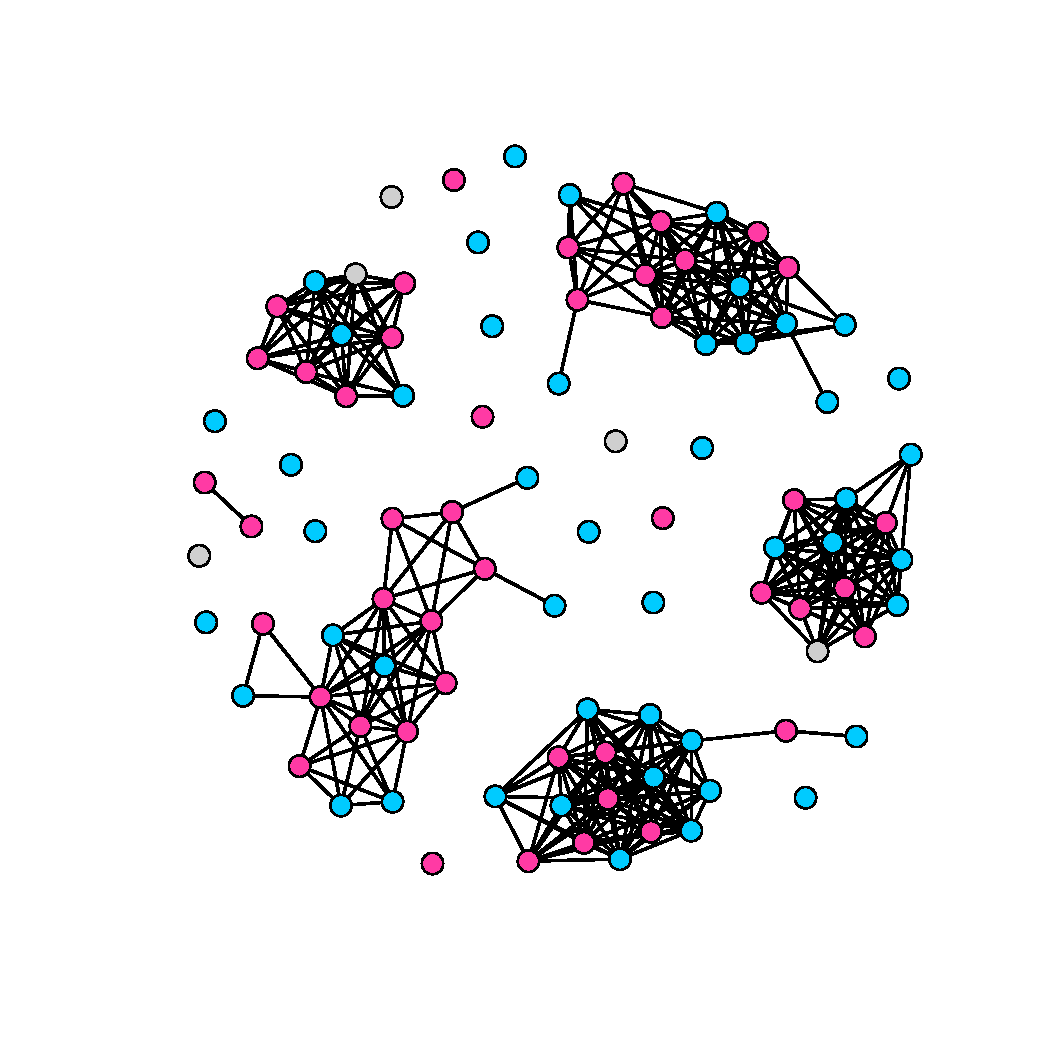
\includegraphics[width=.45\textwidth]{assets/pdf/graph_january_30h_gender.pdf}
				}
	\caption[Network visualizations for June 2008 and January 2009]{Network visualizations for June 2008 and January 2009.}
	 \label{fig:june_jan_side}
\end{figure} 

The amount of edges between the genders is most of the time higher than the amount of edges running within the gender. Moreover, female mice seems to be better connected among each other as males. The most significant differences are found for the networks of January and February. The number of mice is almost equal for both genders for these two months (see figure \ref{fig:long_node}), but the number of edges running between females is noticeable higher. 
      
\subsubsection{Components}

The number of network components (see figure \ref{fig:long_comps}) reveal, how fragmented  the network is. \textit{Isolates} have not been counted as components in this calculation. The values for the female and male mice indicate, in how many network components one or more individual of the gender is found. Therefore, an overlapping of the values for the genders and the value of the number of components (colored blue) indicates a good mixing of genders in the components. This is the case, for instance, from October to December. Consequentely, we may expect disassortative mixing by gender (see section \ref{para:gender_corr}) for these months. The dynamic of the gender correlation coefficient is pictured in figure \ref{fig:long_gender_corr}. Indeed, over the period in question the coefficient $r$ is around 0, which speaks for disassortative mixing.

\begin{figure}[htpb]
\begin{center}
  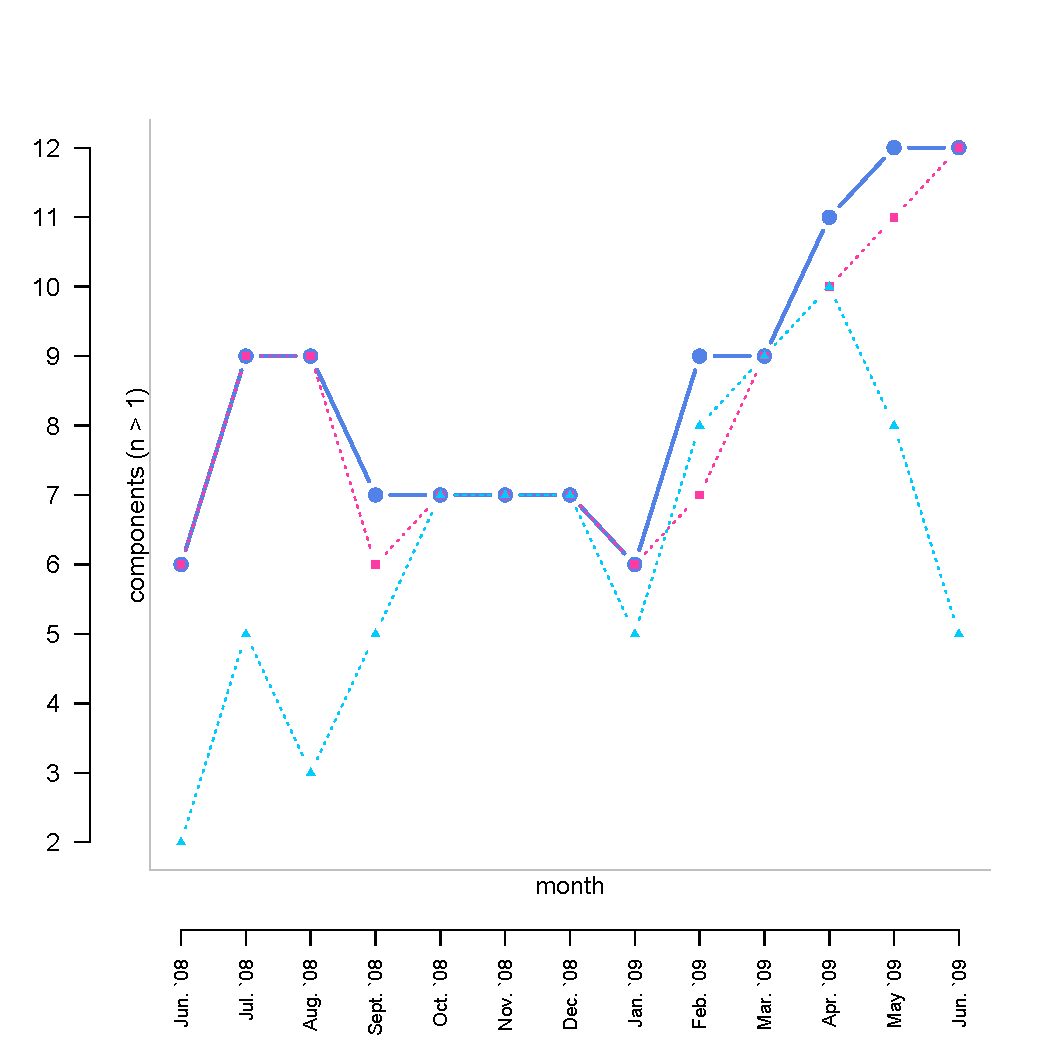
\includegraphics[width=.6\textwidth]{assets/pdf/long_comps.pdf}
  \caption[Number of components over the months]{Number of components over the months. \textit{Isolates} are not included in the calculation.}
  \label{fig:long_comps}
\end{center}
\end{figure}


% \subsubsection*{Clustering coefficient}
% 
% \begin{figure}[htpb]
% \begin{center}
%   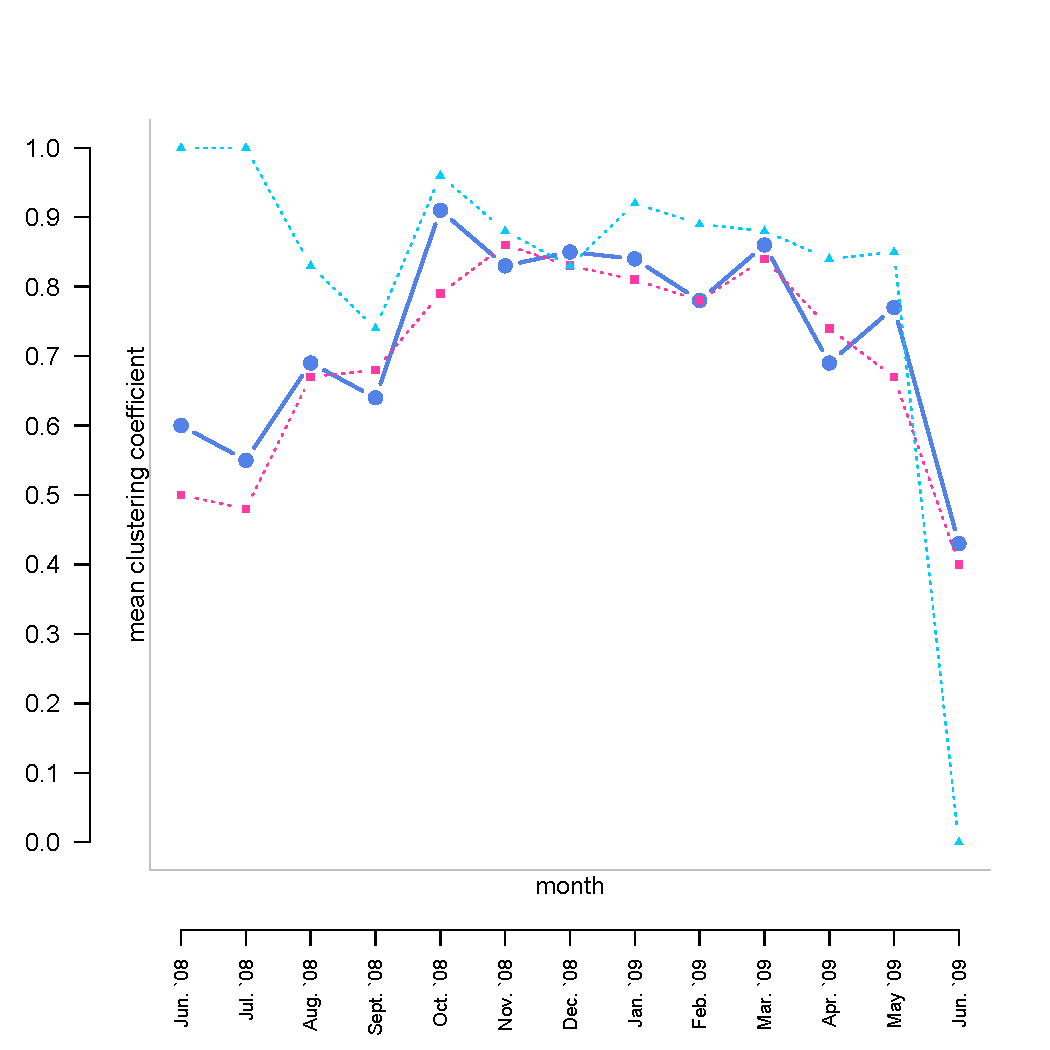
\includegraphics[width=.6\textwidth]{assets/pdf/long_cc.pdf}
%   \caption[clustering coefficient]{clustering coefficient}
%   \label{fig:long_cc}
% \end{center}
% \end{figure} 

\subsubsection{Degree}

Pictured in figure \ref{fig:long_degree} are the mean degrees of the nodes over the months. As already assumed based on the observation made in the single network in section \ref{subsubsec:nbm_dist}, female mice retain a higher mean degree over the whole period. This is another argument that supports the fact, that female mice are socially better or wider connected.

\begin{figure}[htpb]
\begin{center}
  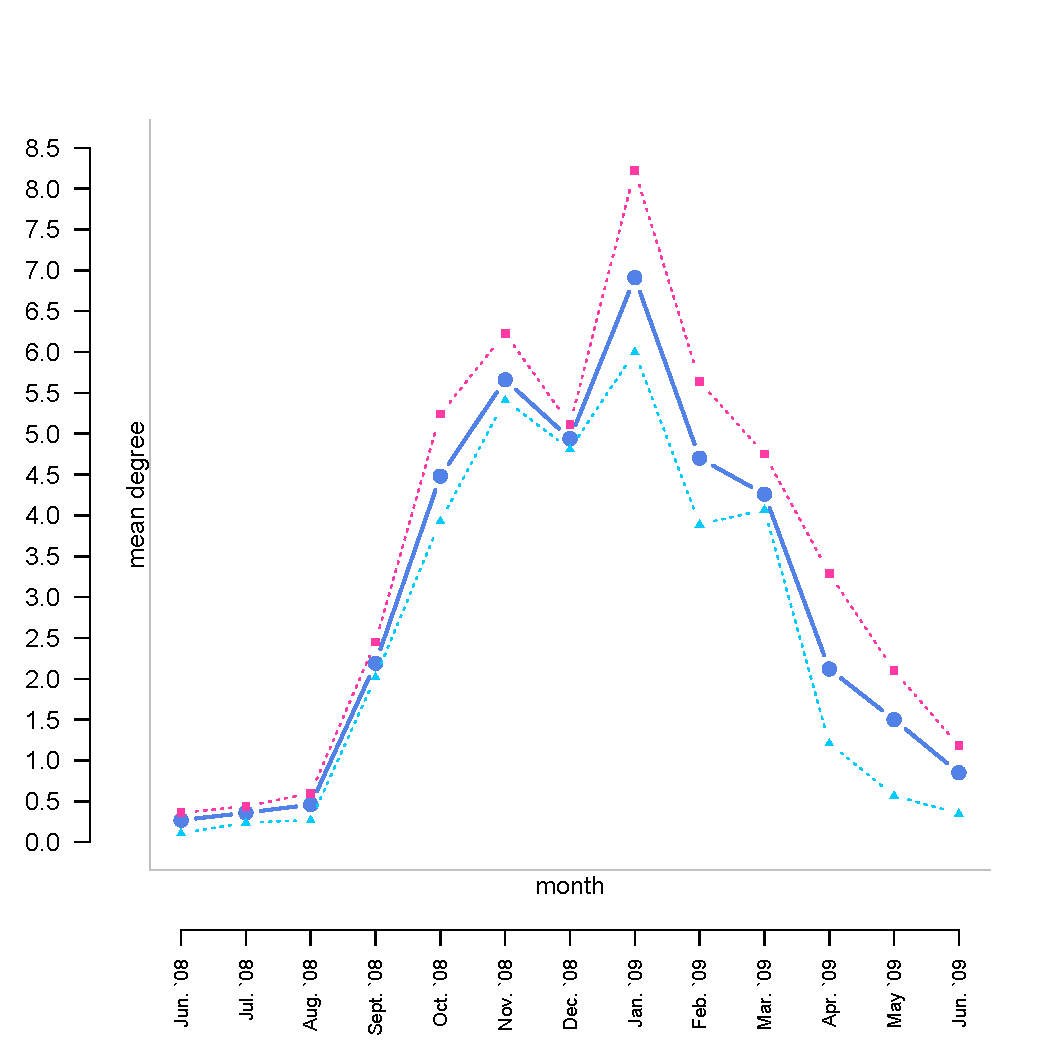
\includegraphics[width=.6\textwidth]{assets/pdf/long_degree.pdf}
  \caption[Mean degree of the nodes over the months]{Mean degree of the nodes over the months.}
  \label{fig:long_degree}
\end{center}
\end{figure} 


\subsubsection{Betweenness}
\label{subsubsec:long_betweenness}

As already mentioned in the section where the betweenness value has been introduced (see section \ref{subsubsec:node_between} on page \pageref{subsubsec:node_between}), the betweenness usually correlates with the degree of a node. The mean betweeness values for the monthly networks shown in figure \ref{fig:long_betweenness}, mostly support this rule. However, the separation of the betweenness values for the genders is more distinct compared to the degree values (see figure \ref{fig:long_degree}). An exception to the rule are the values found in March.   

\begin{figure}[htpb]
\begin{center}
  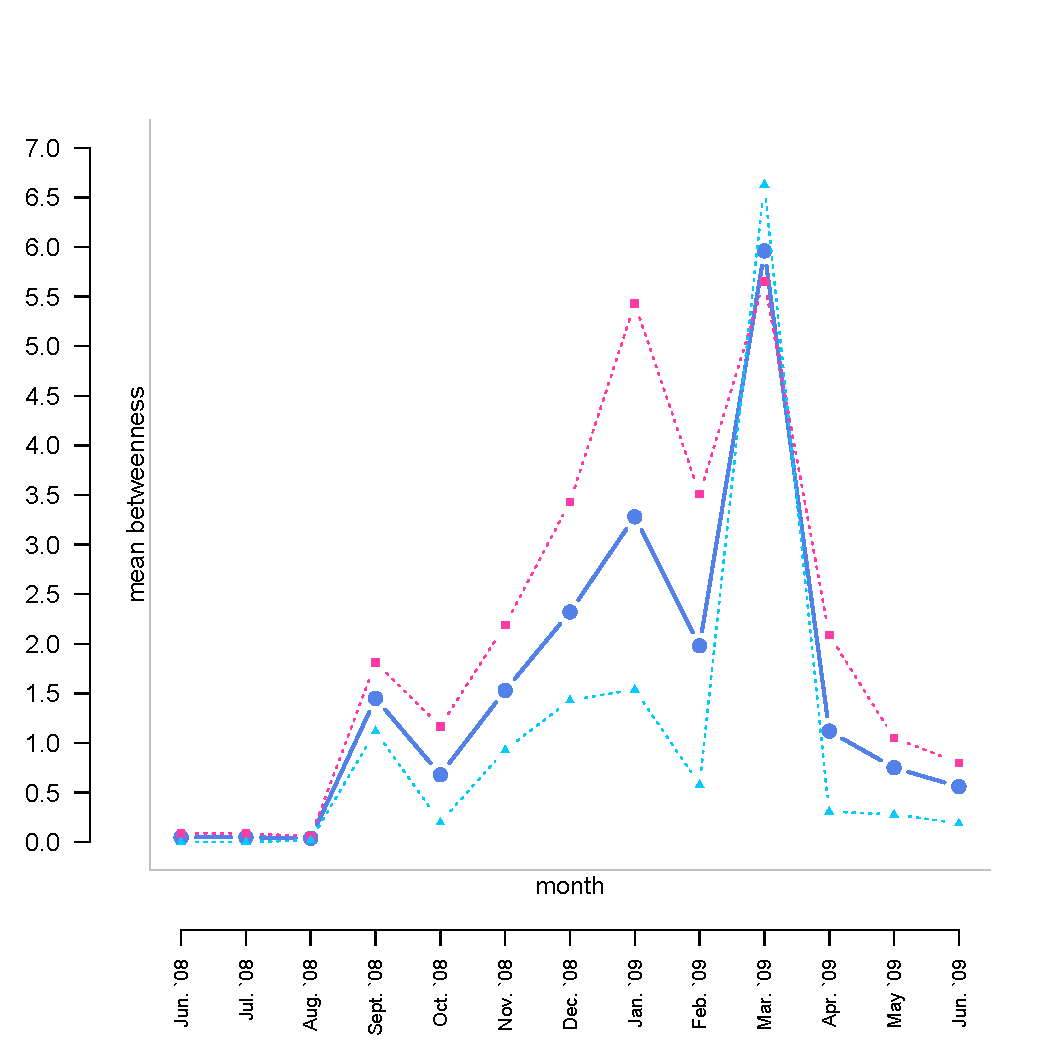
\includegraphics[width=.6\textwidth]{assets/pdf/long_betweenness.pdf}
  \caption[Mean betweenness of the nodes over the months]{Mean betweenness of the nodes over the months.}
  \label{fig:long_betweenness}
\end{center}
\end{figure}

In March, males show a higher mean betweenness than females. Since this observation does not correlate with the mean degree values, we expect some males to be \textit{brokers} according to the definition in section \ref{subsubsec:node_between}. The network visualizations shown in in figure \ref{fig:graphs_march}, identify two male mice with an exceptionally high betweenness value (figure \ref{fig:graph_mar_prop_bet}) which are  \textit{Cut-Points} (figure \ref{fig:graph_mar_hl_cp}) as well. Such nodes, and especially the edges between them, may be of great interest for somebody who plans to analyze single edges in the network.   

\begin{figure}[htpb]% 
	\centering 
	
	\subfloat[Node size proportional to betweenness value]{
					\label{fig:graph_mar_prop_bet}%
					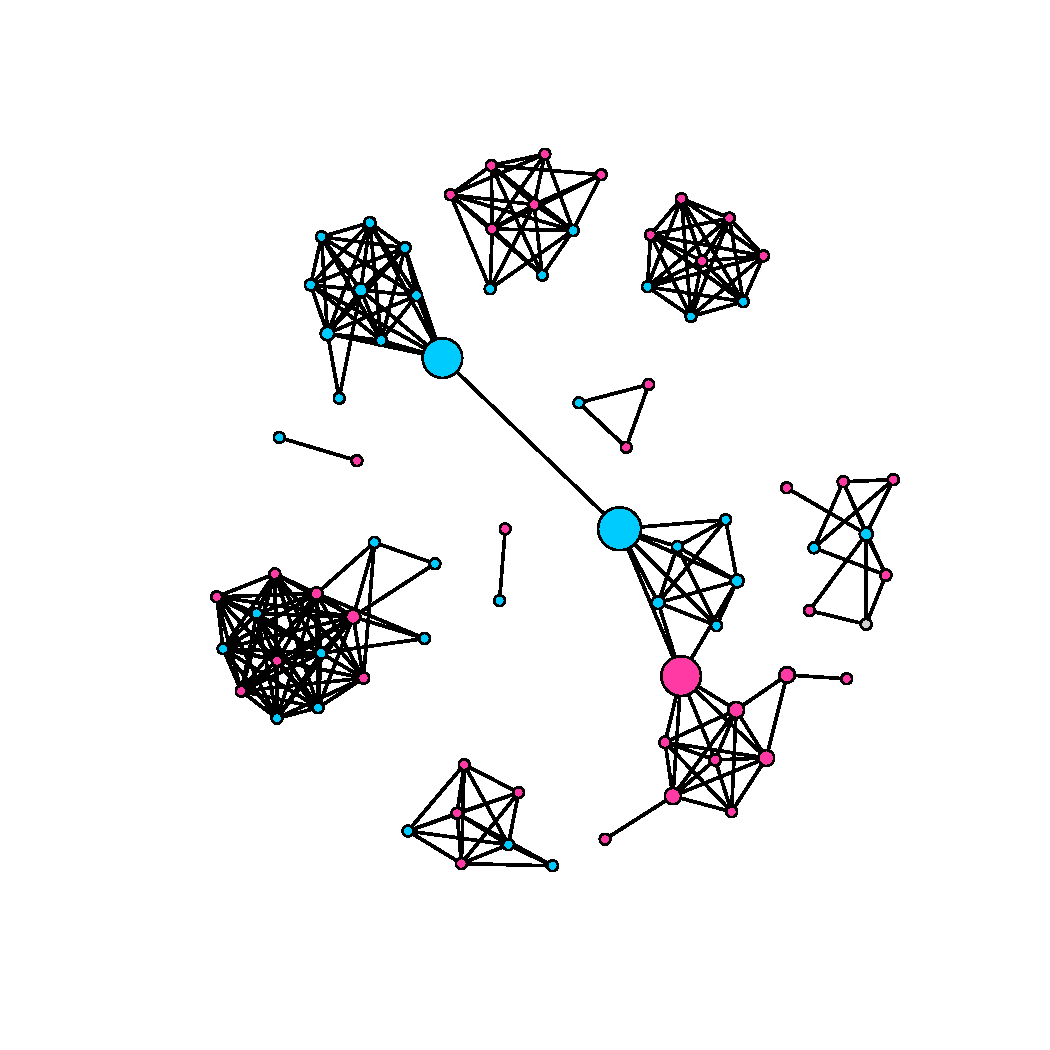
\includegraphics[width=.45\textwidth]{assets/pdf/graph_march_09_30h_prop_bet.pdf}
				}	
	\qquad 			
	\subfloat[Highlighted \textit{Cut-Points}]{
					\label{fig:graph_mar_hl_cp}%
					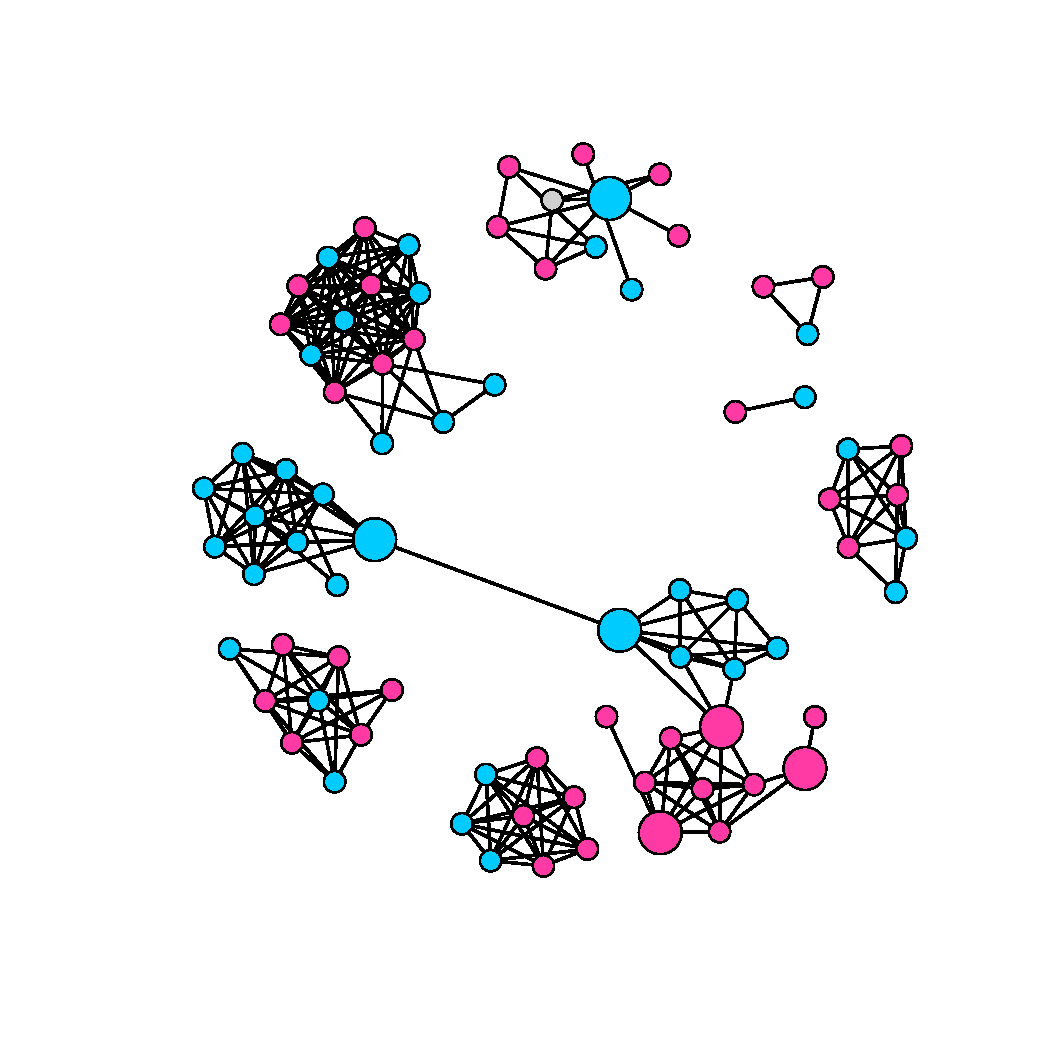
\includegraphics[width=.45\textwidth]{assets/pdf/graph_march_09_30h_hl_cutpoints.pdf}
				}
	\caption[Network visualizations for March 2009]{Network visualizations for March 2009, where the node size is proportional to the betweeness value of the node \subref{fig:graph_mar_prop_bet}, and the \textit{Cut-Points} are highlighted \subref{fig:graph_mar_hl_cp}.}
	 \label{fig:graphs_march}
\end{figure} 


\subsubsection{Gender correlation}

Pictured in figure \ref{fig:long_gender_corr}, are the assortativity coefficients $r$ for the gender correlation. A clear tendency, away from the disassorsative to an assortative mixing is shown. However, $r$ values for sparse networks, as the one of June 2009 ($\rho = 0.02$), may be doubted to be significant.

\begin{figure}[htpb]
\begin{center}
  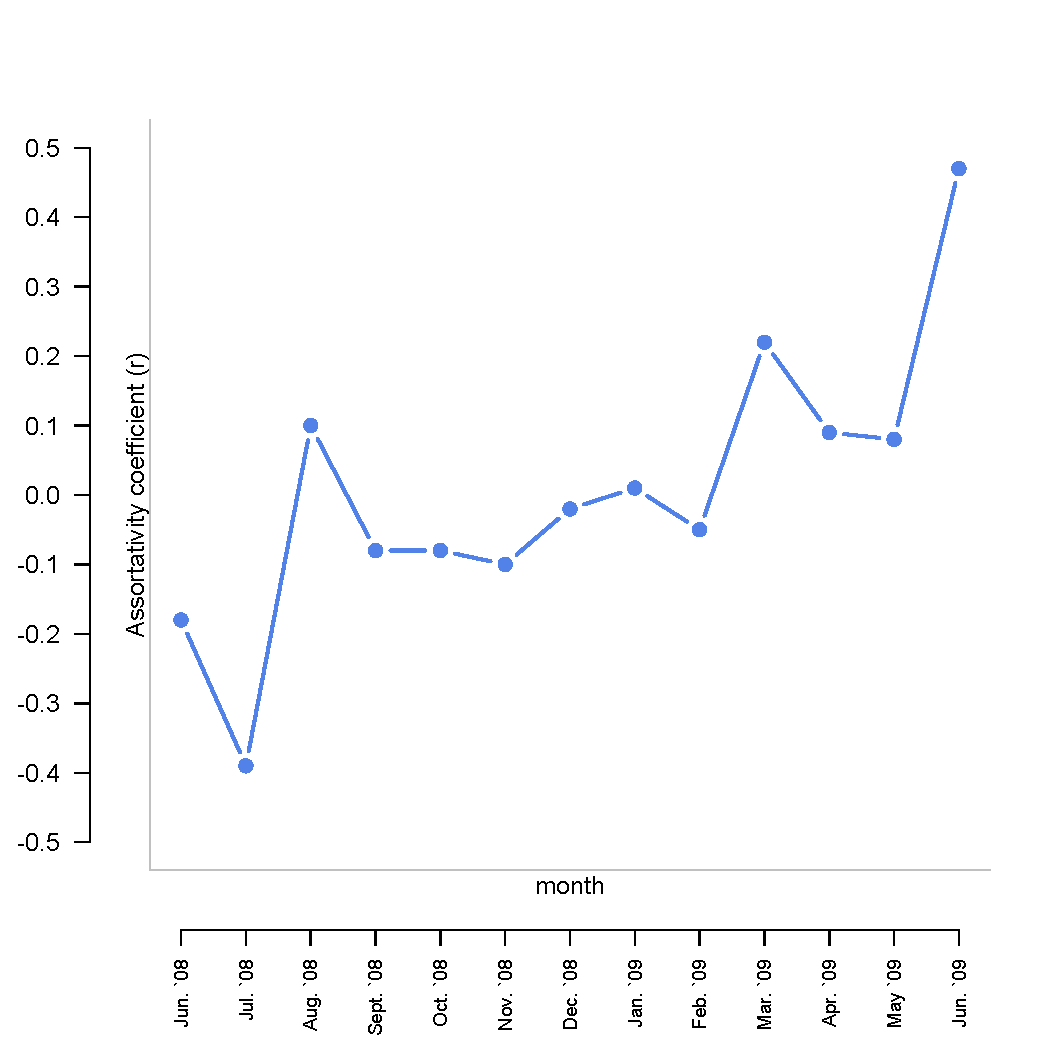
\includegraphics[width=.6\textwidth]{assets/pdf/long_gender_corr.pdf}
  \caption[Assortatitivity coefficient of genders over the monts]{Assortatitivity coefficient of genders over the months.}
  \label{fig:long_gender_corr}
\end{center}
\end{figure} 


\subsubsection{Degree correlation coefficient}

No periodicity, stabilty, not even a tendency is visible in the degree correlations shown in figure \ref{fig:long_degree_cor}. However, the values for the coefficient are positive over all the months, which is consistent with the values determined for other social networks (see section \ref{para:degree_corr}). 

\begin{figure}[htpb]
\begin{center}
  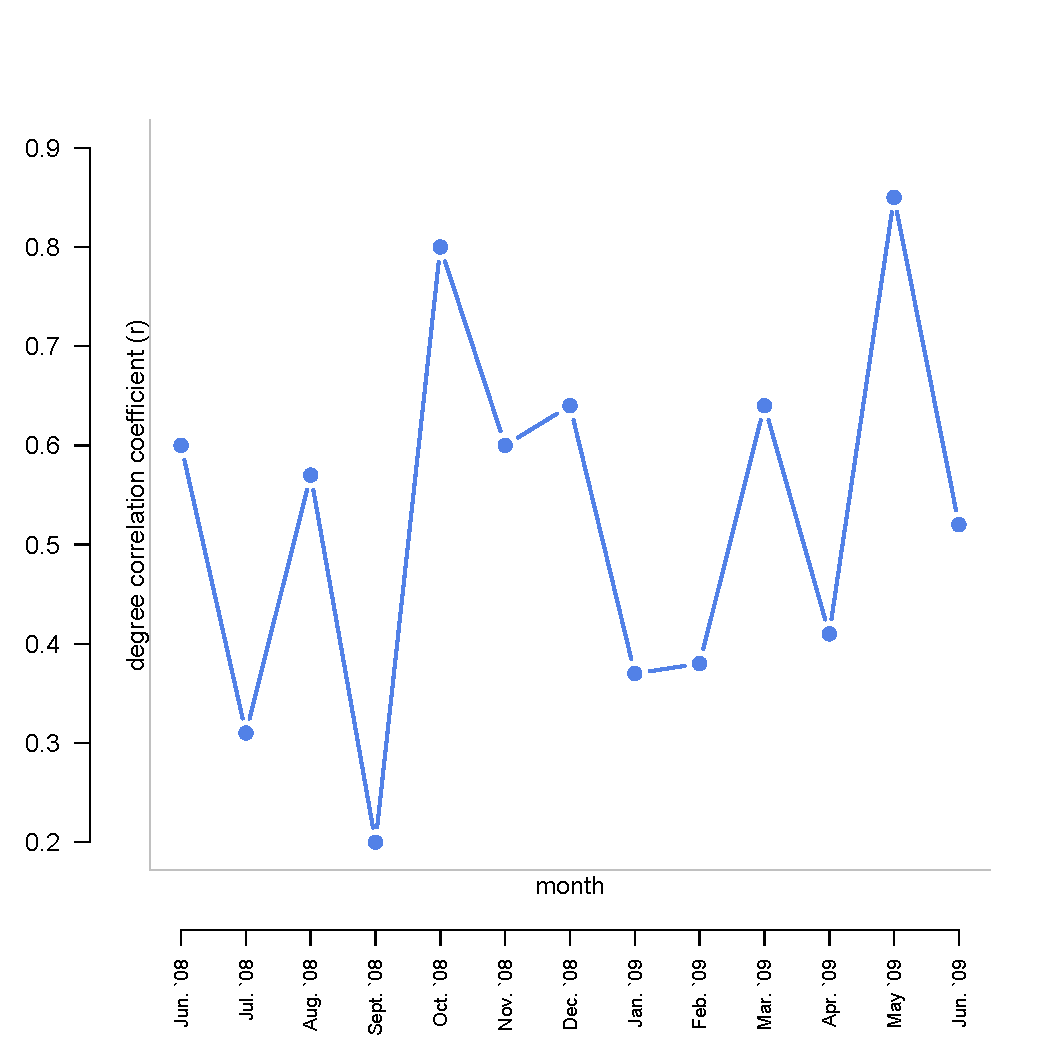
\includegraphics[width=.6\textwidth]{assets/pdf/long_degree_corr.pdf}
  \caption[Degree correlation coefficient over the months]{Degree correlation coefficient over the months}
  \label{fig:long_degree_cor}
\end{center}
\end{figure} 


\subsection{Identifying potentially interesting individuals}
\label{subsec:follow_individuals}

The idea presented in section \ref{subsubsec:vis_individuals}, to identify mice at important positions in the network based on the betweenness values, has been applied to all months with a density $\rho \geq 0.05$. The method to detect these nodes is as follows. At first, the nodes with the five highest betweenness values in the network are shortlisted. Each of the nodes in the shortlist is then removed from the network and the number and size of components before and after the deletion is compared. A node is assesed as a result, if the removal of the node does not create an additional component with size 2 or less. Table \ref{tab:foll_bet} lists the nodes found in the networks.

\begin{figure}
\begin{center}
\scriptsize
\renewcommand\arraystretch{1.5}% (MyValue=1.0 is for standard spacing)
\begin{tabular}{+l|^l|^l|^l|^l|^l|^l}
\hline
\rowstyle{\bfseries}
Sept. `08 & Oct. `08 & Nov. `08 & Dec. `09 & Jan. `09 & Feb. `09 & Mar. `09 \\\hline
0006CC79CA	(m) & 00069552DA (f) & 0006B8D0DF (f) & 0006CD3416 (f) & 0006B9CCE9 (f) & 0006B9BAB9 (f) 	& 0006CD4748 (f) \\
0006B9D3CB	(m) & 0006BA0C9F (f) & 0006B9C5E8 (f) & 0006B8E0D4 (f) & 0006B9D225 (f) & 0006B8CC8C (f) 	& 0006CC69BE (m) \\
				& 0006B9C5E8 (f) & 0006CC62D7 (f) &	&								& 0006CD3416 (f) 	& 0006CD5439 (m) \\
				& 0006B9D225 (f) & 0006CC62BF (m) &	&								& 0006B8E0D4 (f) 	& 0006954D6A (f) \\			
				&	&	&	&	&																		& 0006CC5D4D (f) \\\hline					
\end{tabular}
\captionof{table}{Potentially interesting nodes identified by a high betweenness value for the months between October 2008 and March 2009.}
\label{tab:foll_bet}
\end{center}
\end{figure}

Due to the observations made for the betweenness value (see section \ref{subsubsec:long_betweenness}), it is not surprising, that most of the found nodes are females (14 females and 5 males). A closer look at the table reveals, that some of the mice which occupy such a position, are found in two months (see table \ref{tab:foll_bet_more}). By means of the network visualizations for December and February, shown in figure \ref{fig:pi_nodes_dec_feb}, one can identify the positions of the two nodes (0006B8E0D4 and 0006CD3416) in the network.

\begin{table}
\begin{center}
\scriptsize
\renewcommand\arraystretch{1.5}% (MyValue=1.0 is for standard spacing)
\begin{tabular}{+l|^l}
\hline
\rowstyle{\bfseries}
RFID (sex)	&	Months \\\hline
0006B8E0D4 (f)	& December / February \\\hline
0006CD3416 (f)	& December / February \\\hline
0006B9C5E8 (f)	& October / November \\\hline
0006B9D225 (f)	& October / January \\\hline 													
\end{tabular}
\captionof{table}{RFID's with high betweenness values which are found in two months.}
\label{tab:foll_bet_more}
\end{center}
\end{table}

\begin{figure}[htpb]% 
	\centering 
	
	\subfloat[December 2008]{
					\label{fig:pi_nodes_dec}%
					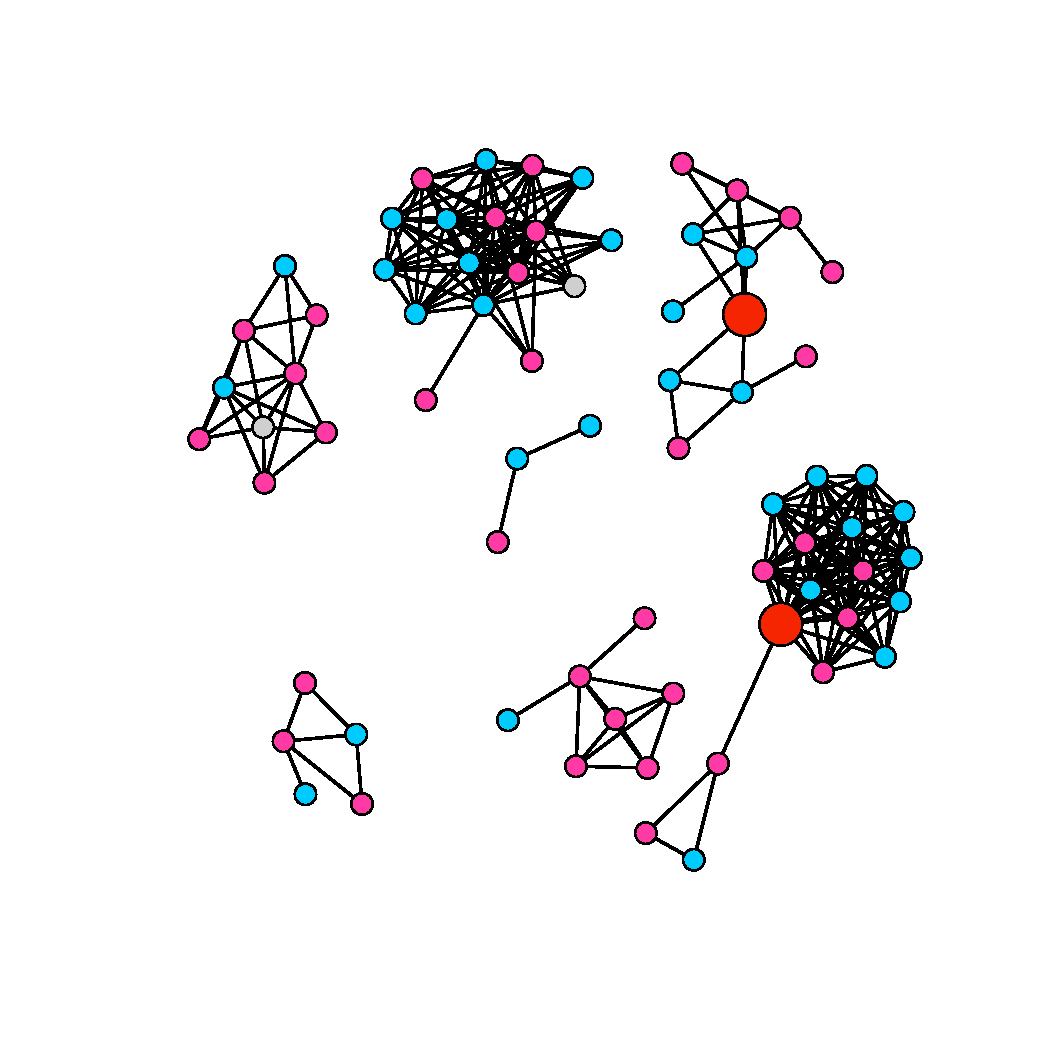
\includegraphics[width=.45\textwidth]{assets/pdf/pi_nodes_dec.pdf}
				}	
	\qquad 			
	\subfloat[February 2009]{
					\label{fig:pi_nodes_feb}%
					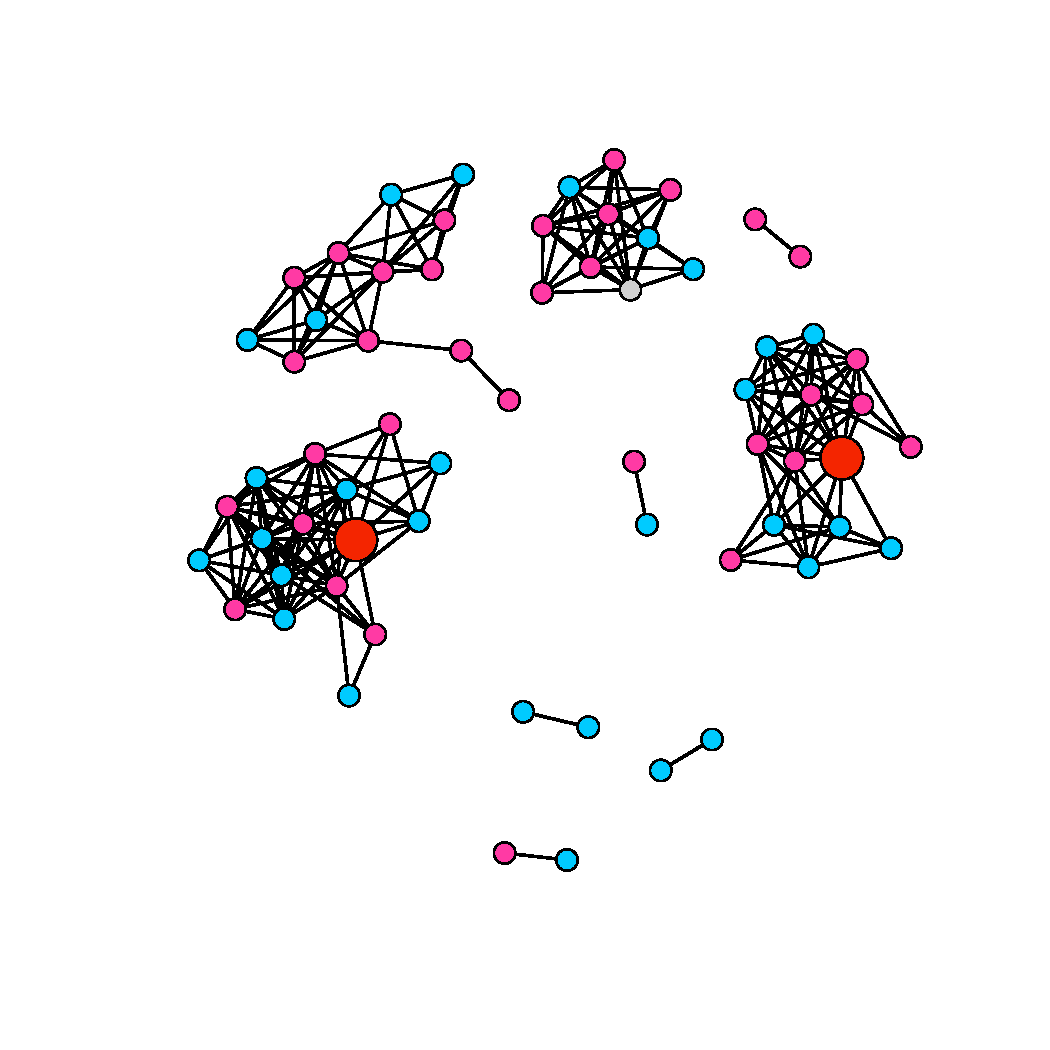
\includegraphics[width=.45\textwidth]{assets/pdf/pi_nodes_feb.pdf}
				}
	\caption[Network visualizations for December 2008 and February 2009 ]{Network visualizations for December 2008 \subref{fig:pi_nodes_dec} and February 2009 \subref{fig:pi_nodes_feb}. Nodes with a high betweenness value found in both months are highlighted red.}
	 \label{fig:pi_nodes_dec_feb}
\end{figure} 

Other approaches are imaginable to identify potentially interesting nodes. For instance, one could choose a mouse based on observations made in the barn, and trace the positions of it in the network. Or the mice which are connected even during the summer could be followed.

\subsection{Discussion}
\label{subsec:discussion}

We showed, that the meetings which led to a network component, are strictly limited to just a few nestboxes. These nestboxes are located in a restricted area of the barn. Therefore we suggest some kind of a nestbox terretory. This raises questions about if and how the reproductional success of female mice depends on such a terretorial behavior. For instance, do females, wich occupy more boxes during winter, show a higher reproductive output in the next spring. Or is the size of the group, or even the network component, an indicator of the reproductive success. However, the group size may depend on on other factors, like the available space in a nestbox, or thermoregulatory aspects, as well.

Interestingly not much components could be found which consist exclusively of male mice. This indicates, that male mice try to dominate a group of female mice. For the female mice in the group, however, we expect formation of social bonds, to share broad-rearing duties like nursing. There is a real possibility that the present network data, paired with the genetical information and observations made in the barn, help to identify reproduction groups. Once they are identified, the social network analysis could contribute to study the dynamics within such a group.     

The observed seasonal variation in the networking of the mice can arise from different reasons. One would be, that the mice spend more time together in the nestboxes to keep each other warm during winter. The energy costs for the thermoregulation are considerably lower if the mice lay close to each other in a covered nestbox laid-out with hew and straw. A second reason could be found in the seasonal discrepancy of the competitive behavior for reproduction. During summer, the competition within male mice to get access to females is high. Wounded males, which are found regularly during these times, are a clear sign for this rivalry. Female mice seem to compete among each other to aquire and defend safe nestboxes, in which they raise their offspring. During winter time, however, the reproductive activity is low. A hypothesis is, that the energy costs to wean a litter and to retain the thermoregulation at the same time are to high, even when food is provided ad libitum. This hypothesis goes well together with the former reason, that the energetic costs of the thermoregulation plays an important role.    

The few edges that exist in the networks during the summer time, primarily exist between females. We assume, that this are collaborative females, which raise their pups in a communal nest. This can be verified, once the gentical data is available.

As already mentionend, the female mice tend to be connected to more indviduals as the males. Furthermore, based on the methods used in this approach, they occupy most of the important positions in the network. However, the weight of the edges has been neglected in the analyzed networks. It would be interesting to carry out the analysis using methods which take the weights into account. The comparison of the results would show, if females are not just better, but even stronger connected.

With the measures and methods used in this approach, the networks have mainly been analyzed as a whole. Few attention has been payed to the individual edges. Although it would be really simple to locate a mouse or a potentially interesting edge using the \textit{miceminer} interface.

In summary, it can be said that the evaluation of the social network contributes to the understanding of the factors that underlie the social structure in this population of mice. In addition, the examination of the network can raise questions, which maybe would never have been asked using conventional methods. The social network approach presented here, includes only a small set of known methods, in a research field which gains more and more attention. Whith that in mind, there are certainly a lot of research questions that can be tackled using the social network analysis, even in biology.
   




